%!TEX ROOT = thesis.tex
\chapter{Literature Review}
\hspace{12.7mm}This chapter reviews the existing literature on machine learning applications for the prediction of cognitive impairment and dementia to provide a foundation for this research. It covers multiple stages of cognitive decline and discusses early detection and classification of different cognitive impairment subtypes. The chapter also includes a critical discussion of the existing research gaps. This review of the literature highlights the need to develop cost-effective, accessible, and explainable machine learning models for the early prediction of cognitive impairment, which is the objective of this research.

\section{Machine Learning and Predictive Modeling in Clinical Science}
\hl{Clinical science is the field of medicine that studies diseases, and it builds knowledge through observation, clinical studies, and the analysis of patient data to guide decisions about diagnosis, prognosis, and treatment} \cite{Sackett1996Evidence}. \hl{A clinical decision is usually reached by collecting different types of information, including the patient history, a physical examination, and laboratory or imaging tests} \cite{Ng2025Clinical}. \hl{These findings are then combined with the experience of the clinician and the available medical evidence to form a diagnosis and a treatment plan.}

\hl{Although clinical science has improved medical care, it still has some limitations. The diagnostic process depends on trained specialists and suitable equipment, and such resources are not equally distributed} \cite{Kwaku2023Prioritising}. \hl{The clinical decision also relies on human judgment, which can vary from one clinician to another and may lead to diagnostic errors} \cite{NewmanToker2024Burden}. \hl{In addition, some diseases develop slowly and show few signs in their early stages. Therefore, the diseases are often detected only at a late stage when the treatment becomes less effective. Such limitations become more serious in low-resource settings, where access to specialists and advanced tests is restricted. These challenges have encouraged researchers to look for data-driven methods that can support clinical decisions and make them more accessible.}

Machine learning (\acrshort{ML}) has become the most common type of artificial intelligence (\acrshort{AI}) in clinical science and healthcare. ML allows machines to learn knowledge from data autonomously, without explicit programming \cite{Alpaydin2020Introduction}. An ML model is a mathematical or statistical function with parameters. This function takes input features and turns them into an output (a prediction). A learning algorithm adjusts the model's parameters during the model training process, which allows the function to capture useful patterns from the training data. After that, the same function is used to make inferences on new data.

The three most widely used classifications for ML techniques are supervised, unsupervised, and reinforcement learning \cite{Morales2022Brief}. The way models identify patterns in the data and make predictions varies among these methods. In supervised learning, the models are trained for prediction using labeled data, while in unsupervised learning, the data are not labeled, and the algorithm is used to learn the patterns present in the data. The other approach, reinforcement learning, involves an agent that learns to take specific actions in an environment to gain the maximum amount of reward. When it comes to model complexity and architecture, ML covers simple models up to ensemble models and deep learning (\acrshort{DL}) models like neural networks. The characteristics of the available data and the objectives of the analysis play a role in selecting the appropriate model. ML is already integrated in various fields and has proven to be particularly useful in healthcare.

ML is increasingly utilized in the healthcare industry to assist medical professionals with analyzing large amounts of medical data in various applications \cite{Habehh2021Machine}. The increasing use of ML in healthcare is due to the accessibility of large and complex healthcare data of various modalities \cite{Krones2025Review}. Furthermore, technological improvement in computational and storage systems has allowed the application of sophisticated ML models in healthcare datasets. In addition, the need to improve the quality of healthcare services and decrease costs has stimulated the development of ML in this field more rapidly \cite{Alowais2023Revolutionizing}.

ML has been used in different fields of healthcare, such as predictive analysis, diagnosis and treatment, and even in the field of personalized medicine \cite{Bajwa2021Artificial, An2023Comprehensive}. Various ML architectures and approaches have been applied to biomedical data from medical images, clinical assessments, Electronic Health Records (EHRs), and other data sources to predict the probability of particular health events \cite{An2023Comprehensive, Binson2024Review}. Healthcare providers and professionals find ML models useful for screening patients with potential risk of chronic diseases like cardiovascular disease, cancer, and diabetes and suggest preventive measures to control the risk. This also helps them make treatment plans more effective and targeted by adjusting the plans based on individual patients \cite{Bajwa2021Artificial}. ML is also used in other healthcare applications, for example, remote patient monitoring, drug discovery, and epidemiological research. As technology continues to advance, ML is likely to improve healthcare outcomes.

Integrating ML into healthcare systems may enable an early and precise disease diagnosis and simplify patient monitoring \cite{Habehh2021Machine}. ML can also automate routine work, which saves medical professionals time and reduces cost \cite{Bajwa2021Artificial}. However, using ML effectively in clinical practice still faces critical challenges \cite{Binson2024Review}. A major challenge is that the data used to train the models can be noisy, scarce, or imbalanced. Medical data often come from various sources and in various formats; therefore, it is difficult to aggregate them for analysis. Moreover, how well the models can generalize to new data and how to interpret complex models are two issues that researchers often do not evaluate or explore \cite{Vermeulen2025Limited}. \hl{Another common limitation is the difficulty of interpreting how complex models reach their predictions, which affects the trust of clinicians} \cite{Martin2023Interpretable}. These challenges reduce the ML models' reliability and raise ethical and legal concerns about the fair and responsible use of ML models in healthcare. Future research work should thoroughly study these concerns and find practical solutions to bridge the gap.

\hl{The prediction of cognitive impairment is one application of predictive modeling in clinical science, and it shares same opportunities and challenges discussed above. The following section focuses on an in-depth discussion of how ML has been used to diagnose cognitive impairment and dementia.}

\section{Applications of Machine Learning in Cognitive Impairment Diagnosis}\label{sec:ml-in-ci}
Cognitive impairment (\acrshort{CI}) is a disorder impacting mental functions and could lead to a decline in memory, language, attention, and problem-solving. CI is a progressive condition that progresses through multiple stages, including mild cognitive impairment (\acrshort{MCI}) and dementia. Dementia represents the most severe stage. At that point, a person may find everyday activities difficult to complete without help. Dementia is categorized as a group of disorders instead of a single disease. It covers a set of conditions that affect cognition, and each condition has its own causes, pathology, and treatment approaches. Therefore, to allow for tailored and more effective treatments, an accurate classification of both the CI stage and the type of impediment is important.

There are risk factors that might appear up to 20 years before the development of dementia and can serve as early warning signs for patients and their caregivers. The majority of these early risk factors are lifestyle and health-related data that are available in primary care units. This indicates that early detection of CI can be made accessible to support timely treatment plans and risk intervention. However, current diagnosis methods fail to serve this purpose because they often cannot detect subtle and mild changes, and they depend on unstandardized tools, specialized equipment, or trained medical professionals. When combined with low awareness, stigma, and financial constraints, early and accurate detection of CI becomes inaccessible for many people, especially in low- and middle-income countries (\acrshort{LMICs}).

ML has been proposed as a scalable screening tool in primary care because it can leverage existing EHRs and simple measurements to flag people at high risk of CI for further assessment. To understand how ML reached this level of applicability in primary care, it is important to trace its evolution in the study of CI and related diseases. Figure~\ref{ml-timelines} presents the timelines of ML in dementia research. In the early years, the field relied on traditional statistical methods to analyze genetic and biochemical factors. These methods helped researchers understand the basic biological mechanisms of the disease. In the first decade of the 2000s, traditional supervised learning models like support vector machine (\acrshort{SVM}) became common. These models were applied to brain imaging and biomarker data for the early detection of CI. Complex methods, like ensemble learning and reinforcement learning, began to be used in the following years between 2011 and 2015. These advanced methods are employed to analyze multimodal data for early detection, predict neuropsychological scores, and study how CI would progress over time. The introduction of DL models brought new potentials to the domain in the following years. These models, when incorporated with new data types, such as advanced imaging, enabled more detailed classification of disease stages and subtypes. More recently, the field has adopted very advanced DL architectures, like time-series models, transformers, and 3D models. These are now used with multimodal data to predict the disease early and to support personalized care plans through explainable AI.

\begin{figure}[ht]
    \centering
    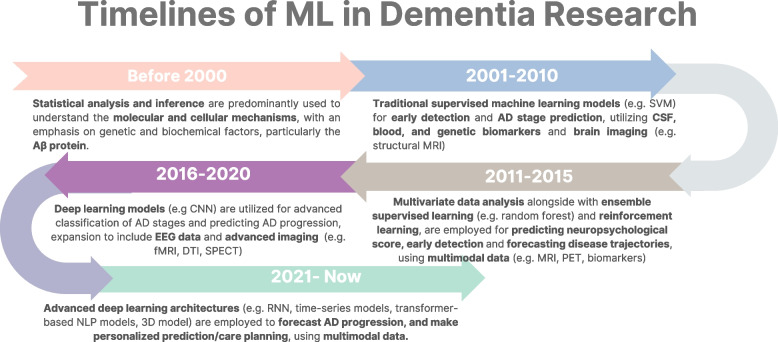
\includegraphics[width=\columnwidth]{figures/timelines-of-ml-in-dementia-research.jpg}
    \caption{Timelines of machine learning in dementia research. This figure is adapted from (Y. Wang et al., 2024, p. 175). Licensed under CC BY 4.0 (http://creativecommons.org/licenses/by/4.0/)}
    \label{ml-timelines}
\end{figure}

Although ML has shown promising results in research, the successful implementation of these ML-based solutions in clinical practice requires careful consideration of data-related challenges, such as ensuring high-quality, diverse, and representative datasets. In addition to addressing ethical concerns, it is crucial to establish robust validation to ensure that the solutions are accurate, reliable, and applicable in real-world settings. The application of ML in dementia prediction is evolving and will continue to grow as more diverse and high-quality data becomes available and the technical and ethical challenges are addressed. The following subsections provide a detailed review of different applications of ML models in CI and related disorders research.

\subsection{Prediction of Cognitive Impairment Using Machine Learning}
Early prediction helps to delay or prevent cognitive decline and promotes timely interventions. It also gives families time to organize support and resources \cite{Alzheimer2025}. Additionally, it may reduce the large social and economic burden on health systems. Recent advances in technology demonstrated that ML can effectively predict CI by analyzing huge amounts of diverse data. This subsection provides a summary of key trends, common challenges, and future research directions from recent reviews, offering a comprehensive overview of the current use of ML to predict CI and dementia.

A recent review systematically analyzed 100 related studies published between 2019 and 2022 \cite{Kaur2024Systematic}. The authors focused on specific types of data, such as Magnetic Resonance Imaging (\acrshort{MRI}), Positron Emission Tomography (\acrshort{PET}), genetic markers, and cerebrospinal fluid biomarkers. A key finding is the overwhelming popularity of DL strategies, which were used in about three-quarters of the studies. While there is an urge to use multi-data approaches, this review found that most researchers still rely on a single data type, specifically MRI scans. The Alzheimer’s Disease Neuroimaging Initiative (\acrshort{ADNI}) database stood out as the most common source of data; concurrently, the convolutional neural network (\acrshort{CNN}) algorithm emerged as the most used and highest-performing model. The review identified a significant gap, as most studies focus on classifying disease states (like Alzheimer’s disease (\acrshort{AD}) \acrshort{vs} healthy) rather than predicting the progression of CI. The paper also made a strong recommendation for researchers to move beyond the ADNI dataset, which would help to avoid bias.

A group of researchers reviewed the literature from the perspectives of doctors and biomedical scientists to provide an overview of ML's role in dementia research \cite{Wang2024Understanding}. They highlighted the history of the field from early genetic studies to today's advanced DL models that can forecast disease progression. This work explored unique methods from the last five years with a wide variety of data, covering simple questionnaires, complex brain imaging, and omics data. Despite the high performance achieved by some studies, serious limitations arise, such as data with missing values, a lack of standard methods for collecting data across different studies, and datasets that do not represent the full diversity of the population. The authors urged global initiatives to standardize the data and improve the clarity of the model predictions for clinicians. 

Another systematic review provides a comprehensive evaluation of automated dementia prediction systems \cite{Javeed2023Machine}. The review categorized studies published between 2011 and 2022 according to the types of data: images, clinical features, and voice recordings. From this modality-based comparison, the authors found that ML models trained on image data, like MRI scans from the ADNI and the Open Access Series of Imaging Studies (\acrshort{OASIS}) datasets, frequently produce better results for dementia prediction compared to models using clinical or voice data. Analyzing various ML techniques, supervised learning models are the most utilized, with SVM being the most frequently used classifier across all data types. Other commonly used classifiers are random forest and CNNs. This review found major problems with the current body of work, such as the possibility of model overfitting and the fact that most of the studies fail to handle imbalanced datasets. The author also highlighted inconsistent methods for training and testing models, which makes it difficult to perform fair comparisons between studies. The review recommends researchers to gather larger and more robust datasets, particularly for voice and clinical-feature analysis, and explore multimodal approaches that combine different data types to create more reliable and efficient prediction models. Similar findings and conclusions were provided by another systematic review \cite{Arya2023systematic}, which encourages reducing the dependence on a single dataset and suggests exploring more diverse data types and combining different models using ensemble techniques.

While most of the reports focus on solutions based on high-cost data, a recent systematic review discussed the potential of automated cognitive assessment using non-neuroimaging data \cite{Babatope2024Potential}. The review selected 87 studies that did not use expensive brain scans like MRI or PET and were published between January 2000 and June 2024. The review concluded that automated tools can produce a comparable level of performance and outperform conventional methods in some studies. To build trust and encourage the adoption of these tools, the authors recommend more collaboration between technology developers and medical experts. 

In a similar context, a more recent review looked at 60 peer-reviewed articles on non-invasive CI detection \cite{Alsuhaibani2025Review}. This review pointed out that models based on speech and language analysis are as effective as those based on costly medical imaging. However, making these automated and low-cost solutions available in low-income regions remains a challenge. Future studies should understand and overcome the barriers that prevent their use in underserved populations worldwide.

Based on this board view of the literature, it can be noticed that there is a clear need for more research and development in the prediction of CI using ML to create affordable and accessible solutions. The following subsections discuss in more detail how different data types are used in the literature to develop ML models for CI and dementia.

\subsubsection{Cognitive Impairment Prediction Using Neuroimaging Data}

Neuroimaging data, such as MRI and PET, are widely used in dementia research. These data offer large shared repositories for training models and contain high-dimensional patterns for analysis. The application of ML in neuroimaging for dementia diagnosis was the subject of a systematic review that surveyed 255 studies \cite{Borchert2023Artificial}. This research area has grown quickly since 2017. This growth coincides with a shift from simpler SVM models to more complex neural networks. This could be related to the introduction of the Transformer architecture in 2017 \cite{Vaswani2017Attention}, which brought scalable attention-based modeling and made it easier to train large, flexible networks on complex data. A great variation in model performance was observed. For instance, the diagnostic accuracy for AD ranged widely from 60.2\% to 99.3\%. Meanwhile, a narrative review paper explored the role of AI and ML in the use of neuroimaging to predict early AD \cite{Rudroff2024AI}. The studies showed a common pattern of use, as CNNs were typically utilized for image analysis, while RNNs were applied to longitudinal data. The review noted a high overall performance. Some frameworks achieved 93\% accuracy in classifying AD and 82\% accuracy in predicting MCI-to-AD conversion by using multi-modal DL.

A systematic review with a meta-analysis focused on the use of multimodal neuroimaging data with ML to classify AD stages \cite{Odusami2024Machine}. The review included 47 studies from 2016 to 2022. Among the different methods, supervised learning algorithms were identified as the most common approach. The authors also highlighted the use of feature-level fusion as a popular strategy to combine various data types from different sources. As a result,  model performance was improved through the use of multimodal neuroimaging data. For classifying AD, the sensitivity was 94.6\% and the specificity 93.5\%. However, the performance in distinguishing progressive from stable MCI was lower, with sensitivity and specificity at 80.4\% and 81.4\%, respectively.

The reviews commonly observed a dominant use of certain brain scans (MRI and PET) and a heavy reliance on the ADNI dataset. Limitations in the reviewed studies were also highlighted, particularly the absence of external validation and the lack of explanation of complex models. The authors suggested several priorities for future studies, including validating models on external datasets, using methods to make AI decisions more transparent, and expanding research into under-studied areas like non-AD dementias.

A group of researchers has developed a DL model for the differentiation of normal cognition, MCI, AD, and non-AD dementias \cite{Qiu2022Multimodal}. They employed a mixed method analysis of data from eight cohorts for developing and testing various models in a multimodal manner. These included an MRI-only CNN, traditional ML classifiers, and a fusion model that combined imaging and non-imaging data. The models showed high diagnostic performance, which is almost equal to that of expert neurologists or neuroradiologists. 

Several studies employed advanced methodologies and neuroimaging data to achieve different objectives. To classify Parkinson’s disease (\acrshort{PD}) using Single-Photon Emission Computed Tomography (SPECT) images, one study proposed a soft attention-based DenseNet model \cite{Thakur2022Soft}. The DenseNet-121 architecture with a soft attention block was used to enhance attention in relevant areas of the brain. The proposed model outperformed previous studies by achieving a high accuracy of 99.2\%. \citeA{Lim2022Deep} built a DL model for early AD diagnosis using structural MRI (\acrshort{sMRI}) data. sMRI scans were preprocessed to remove the skull, correct for the bias field, segment images into tissues, and extract 2D slices from 3D MRI volumes. To overcome the problem of overfitting a small dataset, the authors augmented the data by rotating and zooming the images. The preprocessed images were then used to train and evaluate three CNN models: CNN from scratch, VGG16, and ResNet-50. The VGG16 and ResNet-50 models used transfer learning by initializing the weights with ImageNet pre-trained weights. The VGG16 model produced the most accurate performance of approximately 79\%. Another group of researchers addressed the same problem using a novel DL framework for the classification of early-stage AD based on brain MRI images \cite{Hazarika2023Novel}. The authors employed 3D MPRAGE MRI scans from the ADNI dataset and extracted 2D slices from the hippocampal region. The authors proposed a modified VGG-199 model with Dense and Inception blocks to reduce the number of parameters by 21\%. They then used the Principal Component Analysis (\acrshort{PCA}) to retain 88\% of the original features while retaining 100\% variance. Finally, the classification of cognitively normal, early-stage AD, and AD subjects was performed using a random forest classifier. This method outperformed several state-of-the-art methods with a high classification accuracy of approximately 98\%. The outcomes of these studies prove the possibility of the early diagnosis of CI using brain scans. However, the authors highlighted limitations due to data scarcity and suggested the use of more extensive and diverse datasets, incorporation of multimodal data, and exploration of 3D CNN architectures to improve the model's generalizability and robustness.

A multi-modal approach that combines 3D MRI and amyloid PET scans was implemented to improve AD detection \cite{Castellano2024Automated}. After evaluating different variations of CNN architectures and imaging dimensionalities, parallel processing of multi-modal scans using the dual-branch fusion model achieved the highest results of 95\% accuracy. To address challenges in the early diagnosis of AD from 18F fluorodeoxyglucose (\acrshort{FDG}) PET scans, another paper introduces a novel DL model named ResGLPyramid \cite{Rehman2024Early}. The model is built of a combination of a Tri-Convolutional-Transformer and an attention module. This design allows the model to capture local details and global context from the brain images. The model scored a 92.75\% accuracy and a 0.925 area under the curve (\acrshort{AUC}) for classifying AD and MCI.

Systems based on MRI and PET scans could be used to accurately detect CI. However, the cost and the need for specific equipment and skills prevent many people from accessing these tools \cite{Geethanath2019Accessible}. Researchers have explored the use of electroencephalograms (EEGs) as alternative brain scans to predict CI with ML. EEG is an inexpensive and portable neuroimaging method compared to other methods, such as MRI. Resting state EEG and sMRI were compared in order to differentiate between AD and MCI using low-cost approaches \cite{Farina2020Comparison}. The EEG markers used are frequency band power and functional connectivity. Compared to sMRI, AD classification using EEG achieved a higher accuracy of 70\% with a sensitivity of 74\% and a specificity of 64\%. However, both techniques demonstrated moderate accuracy in differentiating MCI from healthy controls.

A recent review discussed how EEG is used as a diagnostic tool for AD between 2000 and 2023 \cite{Ehteshamzad2024Assessing}. The review found a clear progression. This progression was from traditional visual inspection of EEG to automated analyzes using quantitative EEG (qEEG) and ML. EEG can detect minor functional brain changes much earlier than the structural changes that might appear on MRI or PET scans. Another methodological analysis found that 85\% of studies use EEG signals to detect AD rather than early prediction \cite{Modir2023Systematic}. Additionally, the majority of the studies are using ML classifiers like SVM. These modern approaches can achieve high diagnostic sensitivity and specificity rates above 85\%. The use of EEG signals with more complex models (DL models) for the detection of AD and MCI was recently reviewed \cite{Acharya2025Deep}. The review noted an increase in publications since 2022. This could be driven by the effectiveness of CNNs and transfer learning models like ResNet, which achieved outstanding performance. The use of small datasets and the lack of standardization in EEG protocols are the main methodological gaps highlighted in all reviews.

Access to this effective technology is challenging in LMICs due to the lack of expertise and digital infrastructure. A recent systematic review discussed the potential of automated cognitive assessment approaches that do not rely on neuroimaging data \cite{Babatope2024Potential}. The review included 87 studies that utilized game-based tools, digitized versions of conventional tests, original computerized batteries, virtual reality or smart home systems, and artificial intelligence-based methods. The potential of these non-neuroimaging approaches can be observed from the achieved comparable performance of greater than 80\%. The following subsections provide a review of the application of other effective and more accessible data types in CI prediction.

\subsubsection{Cognitive Impairment Prediction Based on Activity Recognition}
With advances in technology, several automated and noninvasive methods have been developed to predict CI. Activity recognition in intelligent environments, such as smart homes, has been utilized to monitor patient activities to predict CI patterns \cite{Khan2021Prediction}. Digital biomarkers captured by specific human body functions and tasks, such as eye tracking, handwriting, speech, and gaming, have also been employed in dementia prediction research \cite{Ding2022Digital}. 

A recently published systematic review analyzed 72 studies published between 2012 and 2022 that used DL for the diagnosis of dementia using speech and language data \cite{Shi2023Speech}. The review found that many studies have been published in this research domain after 2020. Studies in this field commonly use the DementiaBank dataset. They also often use feature extraction with DL embeddings like Bidirectional Encoder Representations from Transformers (\acrshort{BERT}). The reviewed studies reported high classification accuracies between 80\% and 90\% to classify dementia patients from healthy controls, with some reaching as high as 97\%. In addition to speech processing, \citeA{Alsuhaibani2025Review} reviewed 60 studies that used DL to find CI using non-invasive signs like language, speech, facial expressions, and motor mobility as less expensive alternatives to neuroimaging. Speech- and language-based methods generally achieve the highest detection performance, especially when they combine acoustic and linguistic features. These methods depend a lot on transfer learning with pre-trained models like BERT for linguistic analysis and CNNs or vision transformers for visual data. These reviews pointed out critical gaps that could impact the clinical adoption of these solutions. For instance, large and balanced datasets are limited and standardized data collection methods and model explainability are not applied.

A comparison of speech and gait analysis methods was the focus of another systematic review \cite{Al-Hammadi2024Machine}. It examined 40 studies published from 2017 to 2022. This paper highlighted that SVM was the most common method, followed by DL approaches. This contradicts the heavy focus on DL in other reviews. It was also found that better accuracy can be obtained by analyzing the gait features of the entire body. Future work should explore multimodal approaches (such as fusing gait and speech data) and more diverse languages and longitudinal study designs.

Several studies used natural language processing (\acrshort{NLP}) for the early detection of CI. For instance, \citeA{Amini2024Prediction} developed a new method to predict the progression of MCI to AD within a time frame of 6 years based on speech data and NLP. The approach included three main components: an automated speech-to-text pipeline, a transformer-based sentence encoder to generate embeddings, and finally logistic regression models for prediction. The proposed approach was found to be more accurate than traditional neuropsychological tests and other noninvasive approaches. Other researchers have investigated the optimization of this approach using GPT embeddings \cite{Runde2024Optimization}. The results demonstrated that the transcriptions performed by AI services had better accuracy and F1-score than manual transcriptions. The study showed that NLP can accurately identify AD. However, it was less effective in detecting possible AD and MCI. The authors believe this was due to limited training data.

Looking at different types of digital biomarkers, \citeA{Pavisic2017Eyetracking} built an ML classifier with 95\% accuracy to diagnose early-onset Alzheimer’s using data collected from eye-tracking experiments. In addition, \citeA{Opwonya2023Eye} explored the potential of eye movement data and a multimodal approach to identify MCI in a cost-effective manner. Researchers have built ML models that incorporate eye movement metrics, demographic information, and cognitive scores. While acknowledging limitations in generalizability and the need for further validation, the authors propose this method as a promising, noninvasive, and cost-effective MCI screening solution. As an advance of this approach, \citeA{Alsuhaibani2024Mild} introduced a DL model for the identification of MCI in an early stage based on facial and interaction features obtained from video recordings of patient interviews. The method includes a convolutional autoencoder that extracts holistic spatial facial features from individual frames and a Spatial-to-Temporal Attention Module that captures temporal information and interaction dynamics across video sequences and segments. The framework had an accuracy of 88\% in differentiating MCI from participants with normal cognition, but had the drawbacks of manual video quality assessment and a relatively small dataset.

Using a different approach, another group of researchers developed a novel model to automatically detect dementia based on the dynamics of the handwriting process \cite{Angelillo2019Attentional}. \citeA{Carina2023Handwriting} conducted a systematic review and found that people with AD struggle with various aspects of handwriting. Their review revealed that patients have more trouble with understanding where to place letters on paper and expressing their thoughts through writing compared to simple motor issues. Although the model provides an accurate, cost-effective, and convenient diagnostic solution, its generalizability remains questionable.

In later work, \citeA{Uddalak2024ML-Powered} aimed to detect AD early by utilizing ML to analyze handwriting and take advantage of the effects of AD on fine motor control. Several base classifiers are integrated using the stacking technique to create an ensemble model. The ensemble model was trained on a dataset of handwriting samples gathered from 89 AD and 85 healthy participants. The ensemble model achieved high performance with a 97.44\% F1-score, outperforming the state-of-the-art models on the same dataset. The outcome highlights the considerable clinical utility of ML for highly accurate, cost-effective, and non-invasive prediction of AD through handwriting analysis. 

Other researchers have developed gamified assessment tools to simplify and accelerate cognitive assessment. According to a recent scoping review \cite{Chen2025Video}, these systems demonstrated diagnostic performance comparable to traditional screening tools like the Montreal Cognitive Assessment. In a recent study, \citeA{John2023Development} investigated how ML classifiers could predict cognitive function using head kinematic data from virtual reality exergames. The participants were older adults, and the study took place over a period of six weeks. The classifiers successfully identified correlations between the kinematics of head movement and cognitive performance measures. The findings of this study suggested that virtual reality head movements captured from games can be used as a digital biomarker to assess cognitive status. Gamified systems are engaging and can be used for home monitoring. However, it has been revealed that current research in this area has methodological issues related to small sample sizes and a lack of robust validation methods to assess how these systems work over time \cite{Chen2025Video}.

Although studies leveraging body functions and digital biomarkers offer fully automated, noninvasive, and cost-effective methods for CI and dementia assessments, future work may involve validating the models in larger and more diverse populations and exploring the incorporation of other biomarkers for improved accuracy. Furthermore, the application of these methods may require a certain level of user knowledge, the utilization of specific equipment, and modifications to the patient's environment. These requirements make these solutions impractical and less desirable for conducting highly scalable CI assessments.

\subsubsection{Cognitive Impairment Prediction Using Clinical Notes Analysis}

Examining patterns in clinical notes could be effective in detecting CI. This was the finding of a systematic review of 18 studies using NLP models \cite{Shankar2025Natural}. The review highlighted that the models achieved higher results than rule-based algorithms and traditional ML models. A group of researchers explored using NLP to analyze clinical notes of approximately four thousand patients in two cohorts \cite{Penfold2022Development}. They developed 42 cognitive-related concepts through manual annotation of over 10,000 notes. Using \acrshort{LASSO} regression, the model achieved moderate performance with an AUC of 0.67. The researchers needed to manually label huge amounts of data and set up complex NLP systems to implement their approach. \citeA{Laurentiev2023Identifying} examined how NLP could extract information about daily functioning from digital medical records of people with dementia. Their cross-sectional study developed ML models using clinical note text to identify activities of daily living impairments among 441 older adults with dementia. Random forest and SVM models achieved high AUC scores above 0.97. However, the main limitation was that researchers had to manually annotate thousands of notes and rely on specialists to select relevant keywords for filtering.

A recent study used large language models (\acrshort{LLMs}) to detect cognitive decline from available clinical notes in the EHR \cite{Du2024Enhancing}. In this study, annotated note sections from 6,945 clinical documents related to 2,166 patients were used. The researchers tested how GPT-4 and Llama 2 performed compared to traditional ML models. Although GPT-4 performed better than Llama 2, traditional ML approaches performed better than both LLMs. The performance of an ensemble model combining all models (0.921 F1-score) was higher than the performance of an individual model (0.854 F1-score). In a different study, \citeA{Amini2024From} used a transformer-based Universal Sentence Encoder to analyze clinical notes from Massachusetts General Brigham's EHRs. Using two sampling strategies, they achieved outstanding results in distinguishing normal cognition from dementia (0.978 AUC) and moderate performance for normal cognition versus MCI (0.81 AUC). While demonstrating encouraging outcomes, their approach required extensive computational infrastructure and specialized NLP expertise. In addition, these methods depend on very complex text processing and transformer models.

Analyzing patterns in clinical notes offers an automated and non-invasive approach to detect CI and dementia-related disorders. However, studies in this domain have limitations, including heterogeneity in performance metrics and limited external validation across diverse populations \cite{Shankar2025Natural}. Another limitation is that these methods necessitate extensive annotation and complex programs to process text. To overcome these challenges, there is a need to develop more cost-effective methods to use clinical notes analysis in real clinical settings \cite{Shankar2025Natural}.

\subsubsection{Cognitive Impairment Prediction Using Neuropsychological and Cognitive Tests}
The literature has extensively analyzed in various ways the use of neuropsychological tests and cognitive scores as noninvasive and cost-effective predictors of CI. A group of researchers compared the efficacy of molecular and radiological biomarkers and neurocognitive assessments in predicting the progression from MCI to AD \cite{Daou2023Can}. The accuracy of both methods appears to be inconsistent. This variation is likely influenced by which tests are selected and also by the characteristics of the sample. Valuable insights came from biomarkers. However, neurocognitive assessments presented themselves as an alternative that is more accessible and has a lower cost. This was especially true when tests for memory, executive function, or language were combined. A focus for future research, as suggested by the authors, should be on accessibility and cost.

A systematic review examined 37 studies on AI and ML that were used for the evaluation of MCI and dementia \cite{Veneziani2024Applications}. \citeauthor{Veneziani2024Applications} found three main areas where AI could be very useful. The study suggests that AI can help improve traditional assessments, select effective tests, and create new evaluation methods using virtual reality. It appears that ML algorithms, for example, SVM and DL, were more effective than conventional assessment tools. Some mobile screening tests were found to be better than the standard Montreal Cognitive Assessment, and automated systems for semantic verbal fluency showed a high correlation with manual scoring. The review also highlighted other newly developed technologies, such as game-based and virtual reality tests. However, some important problems remain. Most of the studies were based on the ADNI database, which raises concerns about generalizability. A gap was also noted between technical success and clinical utility in the real-world. The tools should be useful to clinicians to simplify workflow rather than being computationally advanced.

In a previous study, \citeA{Grassi2019Novel} worked to develop an ML algorithm to predict the conversion from MCI to AD. It used different available data, such as demographic characteristics, clinical information, and neuropsychological test scores. The algorithm achieved an AUC of 0.88, which indicates a high accuracy in predicting dementia. The algorithm presented a cost-effective solution depending only on non-invasive and affordable measures. In another work, \citeA{El-Sappagh2021Alzheimers} explored cost-effective approaches to predict the progression of AD using ML. They compared five algorithms trained on multimodal time-series data from the ADNI dataset, including demographic data, cognitive scores, and medication history. The researchers made an important breakthrough by incorporating semantically encoded comorbidity and medication features into their early fusion approach, significantly improving the accuracy of prediction. 

Using ML, \citeA{Alshboul2023Application} studied how to use non-invasive indicators for dementia diagnosis. Their study looked at the ADNI dataset. It focused on factors such as Clinical Dementia Rating (\acrshort{CDR}) scores and demographics. The authors found that ML models could accurately classify patients with dementia. This result shows the potential of low-cost cognitive tests in helping clinicians make an efficient diagnosis. In another study, \citeA{Kim2024Using} tried to develop cost-effective screening tools for cognitive decline using neuropsychological assessments. The researchers analyzed 2,863 subjects with cognitive complaints. All subjects completed the Seoul Neuropsychological Screening Battery, which covers five cognitive areas. The researchers trained a random forest classifier. The goal was to identify the most predictive test combinations for distinguishing between dementia and non-dementia cases. The model's performance was 82.42\% accuracy and had a 0.816 AUC score.

Some researchers investigated ways to make the predictions of the model more transparent. This study explored a methodology to create an efficient and explainable tool for predicting the onset of dementia within three years \cite{Beebe-Wang2021Efficient}. The research analyzed longitudinal clinical and cognitive information across multiple domains. The analysis revealed that data from a single recent visit was enough for an accurate prediction, without the need for years of historical data. Model explainability was a key focus, with the SHapley Additive exPlanations (\acrshort{SHAP}) method used to select a small group of highly predictive cognitive tests and also to provide personalized risk explanations for each person. The final simplified eXtreme Gradient Boosting (\acrshort{XGBoost}) model, which used only four short cognitive tests, achieved a test AUC of 0.89. This performance is comparable to using the entire neuropsychological battery. \citeA{Basta2023Personalized} introduced an ML framework designed for personalized screening for MCI in primary healthcare settings. The study used demographic, clinical, behavioral, and Mini-Mental State Examination (\acrshort{MMSE}) data gathered from 763 older adults. The participants were categorized as 277 with MCI, 153 with dementia, and 333 showed no CI. Since the classes are not balanced, a balanced random forest classifier was trained using a nested cross-validation approach to ensure reliable results. To interpret the reasoning of the model, the researcher employed model-agnostic explainability techniques at the group and individual levels. The framework achieved fair performance in distinguishing cognitively healthy participants from those with MCI, with a sensitivity of 74\%. This result was a clear improvement compared to using MMSE alone, which reached only 37.2\% sensitivity. This result shows that it is valuable to integrate readily accessible primary care data with MMSE scores.

The creation of a highly accurate and interpretable ML model for the early prediction of AD was also the objective of a recently published study \cite{Hossain2025Optimizing}. A publicly available Kaggle dataset was used that contained clinical and lifestyle data from 2,149 adults. The features covered a wide range, from demographics and lifestyle to cognitive assessments (including MMSE) and cognitive symptom reports. The researchers developed a stacked ensemble model. This model first combined predictions from the gradient boosting and XGBoost models. Then, a logistic regression model was used to make the final classification of AD versus non-AD. A very high level of performance was achieved, with the final stacked model showing 97\% accuracy and an AUC of 0.97. The SHAP method was essential for the interpretability of the model. It helped to clarify the influence of each feature on the model's output. This work suggests that an ensemble approach can provide excellent predictive performance. In addition, SHAP provides the transparency that is needed for clinical application. However, the study is limited by its use of a single cross-sectional dataset and the model may not generalize to other populations without further validation in diverse datasets. Another study presented similar findings using a comparable group of features taken from the same Kaggle dataset \cite{Mahamud2025Enhancing}. In this research, the authors applied the Synthetic Minority Over-sampling Technique (\acrshort{SMOTE}) to handle class imbalance. They also used Chi-Square and Recursive Feature Elimination (\acrshort{RFE}) methods to select the most relevant features. Moreover, SHAP and Local Interpretable Model-agnostic Explanations (\acrshort{LIME}) techniques were used to explain how the model made its predictions.

ML models trained in neuropsychological assessments and cognitive test scores are often seen as a non-invasive and more affordable solution. However, it is important to note that these assessments may need trained examiners to administer them. They may also show cultural \cite{Puente2015Neuropsychological} or educational biases \cite{Noroozian2014Impact}. These problems limit how widely they can be accessed and how effective they are as routine assessments. For this reason, the clinical use of neuropsychological assessments requires more effort. These efforts are needed to establish standardized processes \cite{Alzola2024Neuropsychological}.

\subsubsection{Cognitive Impairment Prediction Using Routine Clinical Data}
\label{sec:similar-studies}
In light of the constraints that exist in current non-invasive and automated approaches, scholars have explored other accessible and cost-effective solutions for screening and predicting the onset of CI and dementia. This section discussed recent studies that investigated whether low-cost clinical data collected during regular medical treatment, such as sociodemographic, lifestyle, and health measures, could effectively predict dementia compared to higher-cost assessments. Table~\ref{table:ci-review} provides an overview of the reviewed studies, including utilized datasets and features, modeling approaches, and obtained results.

A related study evaluated the accuracy of accessible clinical data from the National Alzheimer’s Coordinating Center (\acrshort{NACC}) to diagnose and predict AD progression \cite{Ren2023Improving}. The researchers created a framework that organized the data according to its level of accessibility. The data were divided into three groups: low-cost data from primary care, medium-cost data from specialist visits, and high-cost data available only in research settings. The primary care data consisted of demographic details, patient medical history, results of physical examinations, and responses to questionnaires. They trained hierarchical and ensemble ML models in the primary care data to distinguish between cognitively normal, MCI, and AD diagnoses. The multiclass random forest model achieved 0.773 accuracy, which improved to 0.815 in hierarchical classification. In a later study, the same group of researchers applied a similar data categorization with semi-supervised ML \cite{Ren2025Identifying}. The researchers gathered data on 4,014 participants from NACC and 36,621 participants from the \hl{generalized dataset}. They categorized the features into three tiers: low-cost (demographics, behavioral surveys, basic assessments), medium-cost (neuropsychological testing), and high-cost (clinical dementia rating (CDR), genetic testing). Low-cost features with longitudinal data achieved an AUC of 0.719 to predict neuropathological cases. The result was comparable to higher-cost single-visit approaches. The key low-cost predictors included the geriatric depression scale, functional assessment measures, and medication patterns. The outcome of these studies demonstrates that accessible, cost-effective clinical data can be used effectively to detect CI. However, the need for longitudinal data collection could limit the application of these models in real-world settings with restricted access to historical data.

Diverse ML and DL algorithms with readily available and easily accessible health records have been evaluated for the classification of CI. \citeA{Li2023Machine} developed predictive ML models using accessible clinical data for CI among 2,226 participants between 60 and 80 years of age. Only 384 (17.25\%) of the participants were diagnosed with CI. The researchers constructed a composite Z-score for cognitive functioning through four standardized tests. They also included 13 affordable demographic, lifestyle, and clinical features like the dietary inflammatory index, glycated hemoglobin, PHQ-9 depression scores, sleep duration, and albumin levels. Then, ten important features were selected using the Boruta algorithm. They used these features to train a generalized linear model (\acrshort{GLM}), random forest, SVM, artificial neural networks, and stochastic gradient boosting models. The models were trained with 10-fold cross-validation on a 70-30 train-test split. The GLM resulted in the highest performance with an AUC of 0.779. The authors noted a lack of external validation and a lack of family history data. \citeA{Cui2024Prediction} conducted a similar study to develop CI classification models based on accessible data from the Chinese Longitudinal Healthy Longevity Survey. The data were divided into a development dataset of 2,138 participants and two external validation datasets of 501 and 746 participants. The researchers used LASSO regression to select features from a set of 34 features. The initial feature set consisted of health and lifestyle data in addition to activities of daily living (\acrshort{ADL}) and instrumental ADL (\acrshort{IADL}) scores. The researchers evaluated logistic regression, SVM, random forest, and XGBoost using 10-fold cross-validation. Logistic regression outperformed the other models with 0.778 accuracy and 0.875 AUC. Further validation in public health practice is needed to confirm the generalizability of the developed models.

In recent years, researchers have been exploring different ways to use accessible data and ML to create affordable screening tools for dementia and related disorders. A study developed a random forest model to predict dementia using both structural and non-structural data from the Electronic Medical Record (\acrshort{EMR}) collected from several healthcare institutions \cite{Ben2020Predicting}. The model reached an accuracy of 0.80 and was described as a non-invasive and cost-effective method to identify the risk of dementia among general patients. A proof-of-concept study compared ML algorithms versus traditional statistical methods for dementia prediction at a 12-year follow-up \cite{Twait2023Dementia}. \citeauthor{Twait2023Dementia} used clinically accessible data from 4,793 participants. The utilized features are demographic data, clinical variables, lifestyle factors, MMSE, and medication. The researchers evaluated elastic net regression, random forest, SVM, and logistic regression models on three different sets of features. These sets are all features, features after Boruta feature selection, and clinically accessible features (excluding MRI features). All models produced similar levels of performance, but the elastic net regression model was better than the other models considering the balance between the sensitivity and specificity scores. The authors highlighted a potential overfitting because assessments used for dementia, such as the MMSE, are also used as input features.

A novel framework based on a transfer learning paradigm was proposed with the objective of creating an explainable and personalized model for predicting dementia risk \cite{Danso2021Developing}. For this, a source model was first trained with data from the large SHARE study, which included 84,856 older individuals. The knowledge of this model was then transferred and its decision boundaries were updated using data from a younger and undiagnosed population of 473 individuals in the PREVENT study. Sociodemographic information, medical history, and lifestyle details served as input features. For model explainability, SHAP was applied to visualize the risk factors responsible for prediction at both the population and individual levels. The research evaluated random forest and XGBoost algorithms and found that XGBoost was better at predicting AD versus non-AD status in the source model, with an AUC of 96\%. The final target model achieved an AUC of 63\% for predicting high-risk versus low-risk status. The performance of the final model could be affected by the small size of the sample from the PREVENT study.

Multiple studies have evaluated the development of ML models based on accessible data, such as EHRs, for the early prediction of dementia multiple years before disease diagnosis. \citeA{Nori2019Machine} developed a gradient-boosting machine model using data from administrative and EHR sources to predict the onset of dementia from 3 to 8 years. A low sensitivity of 0.47 was achieved by the model in the third year, which dropped to 0.15 in year 8. In a similar study, \citeA{Park2020Machine} employed large-scale administrative health data to predict definite and probable incident AD within 1 to 4 years. The study utilized a nationwide population-based cohort of subjects above 65 years. The predictive models produced a reasonable range of AUC values ranging from 0.644 to 0.775.

Recent studies have explored the use of EHRs to predict Alzheimer’s disease and related dementias (\acrshort{ADRD}) one to five years before diagnosis. This includes a recent development of ML models using data from 23,835 patients and more than a million control patients \cite{Li2023Early}. Data included basic demographic details, medical diagnoses, prescriptions, laboratory test results, and vital signs.  The study examined two approaches, which are knowledge-driven features selected by domain experts and data-driven approaches using all available variables. Logistic regression and gradient boosting tree (\acrshort{GBT}) models were trained on both approaches and tested across different prediction windows. They achieved AUC scores of 0.939 for the 0-year window, 0.906 for 1 year, 0.884 for 3 years, and 0.854 for 5 years before diagnosis. However, the method of this study has critical limitations, like sample selection bias and the absence of external validation. A similar study used EHR data from the University of Missouri Healthcare, consisting of 4,012 ADRD cases and 119,723 controls \cite{Akter2025Using}. The dataset included demographic information, behavioral risk factors, vital signs, and several common comorbidities. The team tested six ML methods: GBT, \acrshort{LightGBM}, XGBoost, random forest, logistic regression, and AdaBoost. Among these, the GBT model performed the best. Its AUC scores were 0.809 for the 1-year window, 0.821 for 2 years, 0.822 for 3 years, 0.808 for 4 years, and 0.833 for the 5-year window before diagnosis. It is worth noting that performance showed an improvement with longer prediction windows, which could indicate that using a wider range of historical datasets improved accuracy. However, the performance of the models on other healthcare systems or populations remains questionable because a generalizability test was not performed in this study.

Other studies aimed to predict dementia with a longer prediction period. A longitudinal retrospective cohort study developed ML models to predict incident dementia in 5, 10, and 13-year prediction windows using routinely collected primary and secondary care EHRs \cite{Georgiev2024Predicting}. The study included 144,113 senior adults aged 50 to 102 years in Scotland. Participants were dementia-free prior to 2009 and had follow-ups until 2023. Only 8\% of the participants developed dementia over the period of 13 years. The researchers employed data-driven and clinically supervised feature approaches, including age, deprivation indices, lifestyle factors, modified electronic frailty index, cardiovascular risk scores, laboratory tests, and chronic conditions. XGBoost models were trained using 70-30 random stratified splits with 10-fold cross-validation. Data-driven models achieved slightly higher AUC scores of 0.888, 0.866, and 0.847 at 5, 10, and 13 years, respectively, compared to clinically supervised models. However, the models resulted in lower sensitivity scores below 0.756. For future work, the author suggested externally validating the model to evaluate its generalizability.

Researchers have also applied ML to classify different stages of CI using accessible data. \citeA{Zhu2020Machine} used records from 5,272 participants recruited in hospitals across Taiwan to distinguish four stages: normal cognition, MCI, very mild dementia (\acrshort{VMD}), and dementia. Data were gathered with a 37-item questionnaire that covered demographic information, cognitive tests, measures of daily functioning, and neuropsychiatric symptoms. The researchers compared three feature selection methods, namely information gain, Relief, and random forest. They also evaluated six different ML models. Using information gain for feature selection together with a Naive Bayes classifier produced the best results, yielding an overall F1-score of 0.81 for multiclassification. Stage-specific F1-scores were 0.67 for normal cognition, 0.68 for MCI, 0.71 for VMD, and 0.93 for dementia. In a related study, \citeA{Vyas2022Identifying} trained binary classifiers to detect dementia and multiclass models to classify its severity. This work relied on demographic profiles, cognitive assessment scores, and clinical parameters. To ensure high modeling quality, dementia experts performed data curation. The researchers evaluated random forest and decision tree algorithms with stratified cross-validation. The random forest model achieved the highest F1-scores of 0.93 for binary classification and 0.81 for severity classification.

The following studies approached the classification of multiple CI stages using multiple binary classification models. This study presented an explainable ML approach for predicting MCI and AD \cite{Yue2023Explainable}. The work utilized data from 2,658 participants in the China Longitudinal Aging Study (\acrshort{CLAS}). A wide range of features were used from categories like demographics, daily lifestyle, medical history, and physical examinations. The modeling process involved handling data imbalance with the \acrshort{ADASYN} (Adaptive Synthetic Sampling Approach for Imbalanced) oversampling technique and comparing five methods for feature engineering, ultimately using ReliefF to select 15 key features. To understand the model's decisions, the SHAP method was utilized to visualize each feature's contribution to the prediction at both global and individual levels. AdaBoost was selected as the best model after evaluating nine different classifiers using 10-fold cross-validation. The model performed two separate classification tasks: normal cognition (\acrshort{NC}) versus MCI and NC versus AD. For MCI/NC prediction, the model achieved an accuracy of 89.2\%, while for AD/NC prediction, the accuracy was 99.2\%.

ML models were developed for predicting MCI and dementia onset using accessible sociodemographic and health-related features from the Korean Longitudinal Study of Aging \cite{Oh2024Multivariable}. The research work included 4,975 older adults aged 60 years or older. Out of these participants, 23 developed MCI and 70 developed dementia. The researchers compared nine ML algorithms and addressed class imbalance using weighting mechanisms. The random forest model achieved the best performance for the prediction of MCI (AUC of 0.673), while XGBoost produced the highest results for the prediction of dementia (AUC of 0.819). Another group of researchers established a similar approach using EHR data from the John Paul II Geriatric Hospital in Poland \cite{Richter2025Cognitive}. The data consisted of 144 individuals with MCI, 38 with dementia, and 101 healthy controls. The study utilized cost-effective features, including sociodemographic variables, laboratory test results, comorbidities, BMI, and functional scales. The researchers evaluated ten ML algorithms after applying \acrshort{ANOVA} for feature selection and SMOTE to balance the training data. For MCI versus control classification, the non-linear SVM model scored the highest performance with 0.69 accuracy and 0.75 AUC. For dementia versus control classification, the random forest model demonstrated high results with 0.84 accuracy and 0.96 AUC. The performance of the binary classification models in both studies highlights that classifying MCI cases is much harder than classifying dementia cases. Additionally, the generalizability of these models is limited by the small data size and retrieval of data from a single research center.

Accessible data from the NACC dataset were used by several studies to classify and predict CI. In a previous study, \citeA{Wang2018Early} compared the accuracy of different ML models for the early detection of AD. The models that were tested included feed-forward and Bayesian neural networks, tree-based algorithms, and long short-term memory (\acrshort{LSTM}). Data came from 6,269 NACC subjects. These subjects had probable AD, and conducted between 2 and 12 visits. The LSTM model achieved an average accuracy of 0.835. This score outperforms the other models by 5\%. In their other study \cite{Wang2018Predictive}, \citeauthor{Wang2018Predictive} utilized the historical medical record of the NACC dataset to develop an LSTM model to predict AD status in the next medical visits. The global CDR score was used to define five different AD stages. The results showed that the proposed approach significantly outperformed the classic baseline methods. These studies demonstrated the potential of recurrent neural networks in producing accurate and reliable models by effectively utilizing the temporal and medical patterns extracted from past patient visits. \hl{In a recent study, a deep learning model was developed on longitudinal data from the ADNI dataset to predict cognitive conversion at different years after the baseline, reaching AUC scores between 0.87 and 0.92, while simpler models that rely on fewer variable sets maintained an AUC above 0.80} \cite{Yang2025Prediction}.

Another study also utilized the NACC dataset and ML models to develop a low-cost screening tool for AD trials \cite{Pang2023Predicting}. The tool is designed based on readily available clinical data to predict the transitions from unimpaired to MCI and from MCI to AD. The researchers evaluated different models and feature selection techniques and eventually identified a group of 20 clinical variables that provided precise predictions. The main outcome of their study is a calculator that is easy to use based on the selected variables. The calculator offers a cost-effective and accessible approach to pre-screening trial participants. Another study approached the progression from MCI to dementia differently \cite{Bucholc2023Hybrid}. The authors developed a two-stage framework. This framework utilized cost-effective and non-invasive cognitive scores from the NACC dataset. In the first stage, distinct cognitive decline trajectories were identified using unsupervised learning. The optimal number of clusters was determined using multiple clustering validity indices and fusion-based methods. These trajectories were then incorporated into supervised ML models in the second stage. As a result, an improvement of 6\% in prediction accuracy was observed, compared to models that only rely on clinical scores. This framework achieved an accuracy of 0.875. This was for predicting dementia conversion using data from four time points. \citeA{abbas2024Explainable} recently utilized data from ADNI to externally validate ML models for the classification and prediction of three cognitive stages. The models were trained using demographic, health history, and cognitive assessment features from the NACC dataset. Using Boruta-based feature selection, 21 features were selected, most of them are related to CDR assessment. The SVM model scored the highest performance in external validation with F1-scores of 0.907 for multiclass tasks and 0.728 for four-year cognitive status prediction. The SVM model also outperformed the other models in binary classification and prediction tasks.

Common approaches and conclusions have been observed in the reviewed studies. An important conclusion is the potential for developing accurate and cost-effective CI screening models using accessible data. With regard to data types, the studies employed various data types, like demographic, health, behavior, lifestyle, and cognitive assessments. It has been found that features related to cognitive assessments are the most predictive features compared to others \cite{Ren2025Identifying, Twait2023Dementia, Vyas2022Identifying}. It can also be noticed that researchers mainly used traditional ML algorithms instead of relying on advanced DL approaches. This approach could be sufficient to analyze structured data and suitable for developing simple and cost-effective solutions. On the other hand, common critical limitations have been observed in the reviewed literature work. Some studies utilized data with a small sample size \cite{Richter2025Cognitive}, with the majority using data with a few thousand samples. The lack of enough data samples is especially noticed in positive cases \cite{Li2023Machine, Oh2024Multivariable}. Subsequently, data scarcity may lead models to overfit noise in data instead of learning informative patterns. This particularly may impact the models' ability to correctly classify positive cases of CI. Models trained and tested on data collected from a single research center or medical institution could be biased and might not generalize well to other populations \cite{ Oh2024Multivariable, Richter2025Cognitive, Zhu2020Machine}. Therefore, external validation using sufficient and diverse datasets is required. This was only done in a few studies \cite{abbas2024Explainable, Cui2024Prediction, Danso2021Developing, Yue2023Explainable}.

\hl{The majority of cognitive impairment prediction models are built on data from high-income countries, despite the fact that most dementia cases occur in LMICs. A recent review reported that, out of more than a hundred developed models, only five were built using data from LMICs, namely China and Mexico} \cite{Alshahrani2024Dementia}. \hl{Accessible data, such as IADL, diabetes, and high depressive symptoms, were found informative in those models} \cite{Alshahrani2024Dementia}. \hl{Similarly, few cognitive prediction models achieved high accuracy using IADL, age, and cognitive screening scores from Chinese cohorts} \cite{Cui2024Prediction, Ren2025Using, Ye2025Predicting}. \hl{The importance of IADL scales for the detection of cognitive impairment and dementia was further confirmed by a systematic review that covered eleven LMICs} \cite{Yemm2021Instrumental}. \hl{However, similar to models developed elsewhere, the few LMIC models identified in that review were not externally validated, and models from high-income countries performed poorly in such settings} \cite{Alshahrani2024Dementia}.

\begin{landscape}
\begin{longtable}{|M{0.15\textwidth}|M{0.15\textwidth}|M{0.4\textwidth}|M{0.3\textwidth}|M{0.5\textwidth}|}

\caption{An overview of recent studies that use ML and routine clinical data for the prediction of CI and dementia} 
\label{table:ci-review} \\
\hline
% \textbf{Study} & \textbf{Dataset}$^{\text{a}}$ & \textbf{Feature Set}$^{\text{b}}$ & \textbf{Models}$^{\text{c}}$ & \textbf{Results}$^{\text{d}}$ \\  
\textbf{Study} & \textbf{Dataset} & \textbf{Feature Set} & \textbf{Models} & \textbf{Results} \\ 
\hline
\endfirsthead

\caption[]{An overview of recent studies that use ML and routine clinical data for the prediction of CI and dementia, continued} \\
\hline
% \textbf{Study} & \textbf{Dataset}$^{\text{a}}$ & \textbf{Feature Set}$^{\text{b}}$ & \textbf{Models}$^{\text{c}}$ & \textbf{Results}$^{\text{d}}$ \\ 
\textbf{Study} & \textbf{Dataset} & \textbf{Feature Set} & \textbf{Models} & \textbf{Results} \\ 
\hline
\endhead

\hline
\multicolumn{5}{r}{\textit{Continued on next page}} \\
\endfoot

\hline

\multicolumn{5}{p{1.5\textwidth}}{\footnotesize
The asterisk (*) in the Models column indicates the best-performing model in the corresponding study.
% \begin{enumerate}[label=\alph*),leftmargin=0.3cm]
% \item AGES-Reykjavik: Age, Gene/Environment Susceptibility Reykjavik Study; CHARLS: China Health and Retirement Longitudinal Study; CLAS: China Longitudinal Aging Study; CLHLS: Chinese Longitudinal Healthy Longevity Survey; JPIIGH EMR: John Paul II Institute of Geriatrics and Gerontology Electronic Medical Records; KLOSA: Korean Longitudinal Study of Aging; NACC: National Alzheimer’s Coordinating Center; NHANES: National Health and Nutrition Examination Survey; NHIS-NSC: National Health Insurance Service-National Sample Cohort; OLDW: OptumLabs Data Warehouse; OneFlorida+: OneFlorida Clinical Research Consortium; SCHS DB: Show Chwan Health System Database.
% \item ADL: Activities of Daily Living; APOE: Apolipoprotein E; CDR: Clinical Dementia Rating; FAQ: Functional Activities Questionnaire; GDS: Geriatric Depression Scale; IADL: Instrumental Activities of Daily Living; MMSE: Mini-Mental State; NPI: Neuropsychiatric Inventory; NPI-Q: Neuropsychiatric Inventory Questionnaire.
% \item AdaBoost: Adaptive Boosting; ANN: Artificial Neural Network; C\&R Tree: Classification and Regression Tree; CatBoost: Categorical Boosting; DNN: Deep Neural Network; DT: Decision Tree; GB: Gradient Boosting; GBC: Gradient Boosting Classifier; GBR: Gradient Boosting Regressor; GBT: Gradient-Boosted Trees; GLM: Generalized Linear Model; GPC: Gaussian Process Classification; KNN: K-Nearest Neighbors; LDA: Linear Discriminant Analysis; lightGBM: Light Gradient-Boosting Machine; LogitBoost: Logistic Boosting; LR: Logistic Regression; LSTM: Long Short-Term Memory; MLP: Multi-layer Perceptron; NB: Naïve Bayes; QDA: Quadratic Discriminant Analysis; RF: Random Forest; SGB: Stochastic Gradient Boosting; SVM: Support Vector Machine; XGBoost: eXtreme Gradient Boosting.
% \item Acc: Accuracy; AUC: Area Under the Curve.
% \end{enumerate}
}

\endlastfoot

\cite{Wang2018Predictive} & NACC & Demographics, Health history, Physical info, CDR, \acrshort{GDS}, FAQ, Time intervals & \acrshort{DT}, \acrshort{LR}, LSTM*, \acrshort{RF}, SVM & Predicting AD progression: Acc=0.991 \\ 
\hline

\cite{Wang2018Early} & NACC & Demographics, Health History, Functional Scales & Bayesian Network, C\&R Tree, LSTM*, Neural Network & Classifying CDR scores: Acc=0.835 \\ 
\hline

\cite{Nori2019Machine} & OLDW & Demographics, diagnoses, medications, procedures from claims and EHR data & lightGBM* & Predicting incident MCI: \newline 3-year: AUC=0.710 \newline 8-year: AUC=0.720 \\ 
\hline

\cite{Ben2020Predicting} & Regenstrief Institute EMR & Demographics, Prescriptions, Diagnosis, Medical notes & ANN, RF*, SVM & Predicting incident dementia: \newline 1-year: Acc=0.774 \newline 3-year: Acc=0.735 \\ 
\hline

\cite{Park2020Machine} & NHIS-NSC & Demographics, laboratory values, health profiles, personal/family history, diagnoses, medications & LR, RF*, SVM & Predicting incident AD: \newline 1-year: Acc=0.713, AUC=0.775 \newline 2-year: Acc=0.675, AUC=0.730 \newline 3-year: Acc=0.632, AUC=0.677 \newline 4-year: Acc=0.663, AUC=0.725 \\ 
\hline

\cite{Zhu2020Machine} & SCHS DB & Neuropsychological tests, IADL, NPI, Questionnaire items & AdaBoost, LogitBoost, \acrshort{MLP}, NB*, RF, SVM & Classifying cognitive status (NC, MCI, Vascular Mild Dementia, Other Dementia): Acc=0.810, AUC=0.950 \\ 
\hline

\cite{Danso2021Developing} & SHARE & Sociodemographics, Self-reported medical history, Lifestyle & Transfer-learning using RF and XGBoost* & Predicting dementia up to 14 years: AUC=0.960 \\ 
\hline

\cite{Bucholc2023Hybrid} & NACC & Cognitive/functional tests, Cognitive trajectory classes & Ensemble, \acrshort{KNN}, LR, RF*, SVM & Predicting conversion from MCI to dementia: \newline 3 visits input data: Acc=0.850, AUC=0.601 \newline 4 visits input data: Acc=0.875, AUC=0.756 \\ 
\hline

\cite{Li2023Early} & OneFlorida+ & Knowledge-driven: Diagnoses, medications, vital signs, lab results. Data-driven: Demographics, behavioral data, diagnoses, medications, procedures & GBT*, LR & Predicting ADRD: \newline 0-year: AUC=0.939 \newline 1-year: AUC=0.906 \newline 3-year: AUC=0.884 \newline 5-year: AUC=0.858 \\ 
\hline

\cite{Li2023Machine} & NHANES & Demographics, lifestyle, lab results, medical history, dietary index, depression score, sleep data & ANN, GLM*, RF, SGB, SVM & Classifying CI vs. non-CI: Acc=0.718, AUC=0.779 \\ 
\hline

\cite{Pang2023Predicting} & NACC & Demographics, medical history, medication use, physical and neurological exam findings, clinical ratings, neuropsychological test scores & LR, RF*, SVM & NC to MCI (within 4 years): Acc=0.715, AUC=0.714 \newline MCI to AD (within 3 years): Acc=0.821, AUC=0.805 \newline MCI to AD (within 2 years): Acc=0.853, AUC=0.854 \\ 
\hline

\cite{Ren2023Improving} & NACC & Demographics, patient history, physical exam, behavioral surveys, MMSE & Auto-sklearn, Clustering model, Hierarchical models*, RF & NC vs. MCI vs. AD: Acc=0.815 \newline AD vs. Other: Acc=0.919 \newline NC vs. Other: Acc=0.889 \\ 
\hline

\cite{Twait2023Dementia} & AGES-Reykjavik & Demographics, Clinical variables, Medication use, Lifestyle variables, Cognitive assessment & Elastic Net regression*, LR, RF, SVM & Predicting dementia up to 12 years: AUC=0.720 \\ 
\hline

\cite{Yue2023Explainable} & CLAS & Demographics, Lifestyle, Medical history, Physical examination & AdaBoost*, Bagging, DT, Extra Trees, KNN, LightGBM, RF, SVM, XGBoost & MCI vs. NC: Acc=0.892, AUC=0.957 \newline AD vs. NC: Acc=0.992, AUC=1.0 \\ 
\hline

\cite{abbas2024Explainable} & NACC & Demographics, Health History, Physical measurements, GDS, FAQ, \acrshort{NPI-Q}, CDR & KNN, \acrshort{NB}, RF, SVM* & Classification: \newline NC vs. AD: Acc=0.973 \newline NC vs. MCI: Acc=0.881 \newline MCI vs. AD: Acc=0.866 \newline NC vs. MCI vs. AD: Acc=0.847 \newline 4-year Prediction: \newline NC vs. AD: Acc=0.964 \newline NC vs. MCI: Acc=0.781 \newline MCI vs. AD: Acc=0.767 \newline NC vs. MCI vs. AD: Acc=0.730 \\ 
\hline

\cite{Cui2024Prediction} & CLHLS & Socio-demographics, Health-related variables, Physical measurements, Lifestyle, daily activities & LR*, RF, SVM, XGBoost & Classifying CI vs. non-CI: Acc=0.778, AUC=0.875 \\ 
\hline

\cite{Georgiev2024Predicting} & DataLoch EHR & Demographics, Lifestyle factors, Routine physical measures, Lab tests, Medications, Comorbidities, Outpatient data & Decision Trees, LR, NB, RF, XGBoost* & Predicting incident dementia: \newline 5-year: AUC=0.888 \newline 10-year: AUC=0.866 \newline 13-year: AUC=0.847 \\ 
\hline

\cite{Oh2024Multivariable} & KLOSA & Demographics, socioeconomic status, social engagement, health-related variables, lifestyle, functional status & AdaBoost, CatBoost, \acrshort{GB}, KNN, LightGBM, LR, RF, SVM, XGBoost* & Predicting CI within 2 years: \newline MCI onset: AUC=0.673 \newline Dementia onset: AUC=0.819 \\ 
\hline

\cite{Akter2025Using} & MU Healthcare EHR & Demographics, Vital signs, Behavioral risk factors, Comorbidities, Medical diagnoses & AdaBoost, GBT*, LightGBM, LR, RF, XGBoost & Predicting ADRD: \newline 1-year: Acc=0.978, AUC=0.809 \newline 2-year: Acc=0.974, AUC=0.821 \newline 3-year: Acc=0.974, AUC=0.822 \newline 4-year: Acc=0.970, AUC=0.808 \newline 5-year: Acc=0.970, AUC=0.833 \\ 
\hline

\cite{Richter2025Cognitive} & JPIIGH EMR & Sociodemographics, Lab results, Comorbidities, BMI, Functional scales & AdaBoost, GPC, KNN, \acrshort{LDA}, MLP, NB, Non-linear SVM, QDA, RF*, SVM & MCI vs. NC: Acc=0.690, AUC=0.750 \newline Dementia vs. NC: Acc=0.840, AUC=0.960 \newline MCI+Dementia vs. NC: Acc=0.750, AUC=0.850 \\ 
\hline

\cite{Ren2025Identifying} & NACC & Demographics, Patient history, Behavioral surveys, Neuropsychological testing, Genetic testing, CDR & Clustering with auto encoder, GB, LR, RF, Semi-supervised model* & Classifying CI: AUC=0.719 \\ 
\hline

\cite{Ren2025Using} & CLHLS & Demographics, Life behaviors, ADL, Disease history, Routine blood and plasma biomarkers, MMSE & Balanced RF*, LR, RF, SVM, XGBoost & Predicting cognitive impairment at 3-year follow-up: Acc=0.885, AUC=0.809 \\
\hline

\cite{Ye2025Predicting} & CHARLS & Education, Childhood friendship, Age, IADL, Hukou type, Mobility, Sleep duration, Gender, Residence, Social participation & GBC*, GBR & Classifying CI: AUC=0.832 \\
\hline

\end{longtable}
\end{landscape}

\subsection{Classification of Cognitive Impairment Subtypes Using Machine Learning}
CI, particularly dementia, could be classified into several types. The most common types are Alzheimer’s disease (\acrshort{AD}), vascular dementia (\acrshort{VaD}), dementia with Lewy bodies (\acrshort{DLB}), and frontotemporal dementia (\acrshort{FTD}). These conditions might have various cognitive profiles and progression patterns in various cases. For instance, dementia due to AD is characterized by memory loss as the primary sign, while dementia due to vascular disease is characterized by more severe executive features. Thus, it is essential to distinguish the causes of cognitive dysfunction in patients to make appropriate conclusions about the further treatment process. However, it could be a challenging task to identify a specific CI subtype because of overlapping symptoms. In addition to variability in disease progression and the potential for multiple contributing etiologies (mixed dementia). What makes it even harder is the lack of standardized diagnostic criteria and screening tools. Therefore, better methods are needed to detect and differentiate the causes of cognitive decline at an early stage to guide appropriate intervention plans. In recent years, there have been some attempts made using ML techniques to handle these challenges and increase the classification accuracy. In this section, several studies in this domain utilizing various sources of data, including neuroimaging, biomarkers, and clinical data, have been reviewed.

The classification of CI has been the focus of researchers, especially in classifying the etiology of the condition at the most severe stage (dementia). The majority of the studies have used structural and functional neuroimaging data for the classification of dementia subtypes. \citeA{Chouliaras2023Use} conducted a systematic review of the application of neuroimaging for the early and differential diagnosis of dementia. They stressed the need to diagnose the diseases properly and in the early stage so that clinical management could be effective and treatment modalities could be efficiently worked out. The authors concentrated more on the advantages and disadvantages of different methods of neuroimaging, with more emphasis on MRI and PET in the differentiation of dementia types. They highlighted that additional research based on longitudinal data from multiple centers should be done to enhance the diagnostic accuracy in the early stages. Another systematic review investigated ML neuroimaging classification across dementia types \cite{Borchert2023Artificial}. The authors highlighted an overreliance on the ADNI dataset and structural MRI data. They pointed out other significant methodological limitations, including insufficient algorithm descriptions, lack of independent validation, and minimal representation of non-Alzheimer’s dementias. 

Interesting insight highlighted by a later review of dementia classification studies that utilize major longitudinal datasets, such as NACC and ADNI \cite{Wang2024Understanding}. The central focus of such classification efforts seems to be the differentiation of Alzheimer’s dementia from other types of the disease, including VaD, FTD, and DLB. As input features, the studies often employed metabolomics data, structural MRI, and functional MRI. The studies utilized various ML and DL models with accuracies frequently exceeding 80\%. The authors of the review pointed out some critical limitations. In particular, insufficient external validation threatens the generalizability of the findings. The reliance on expensive neuroimaging techniques could also create a barrier to implementation in some clinical settings. Finally, most of the research focused on binary classifications rather than developing a single, more comprehensive model to classify multiple types of dementia.

\subsubsection{Cognitive Impairment Subtypes Classification Using Neuroimaging Data}
Features related to brain scans are widely used in ML studies of dementia because they give direct, quantifiable maps of the structural and functional brain changes that separate disease subtypes. Cortical thickness data were used to train a hierarchical model that would help discriminate between different subtypes of FTD and AD \cite{Kim2019Machine}. Their approach obtained the average accuracy of 0.758, outperforming non-hierarchical classifiers. The results indicate that hierarchical classifiers can be effective in complex diagnostic tasks. In a later study, \citeA{Ma2020Differential} used a DL approach to distinguish between normal aging, AD, and FTD with an accuracy of 0.883. They emphasized that using multiple scales and multiple types of features and also data augmentation significantly improves the model’s performance. 
 
A major emphasis has been given to the identification of the differential diagnosis between specific types of dementia, especially AD and VaD. Yineng and colleagues used structural MRI features and SVM to differentiate between AD and VaD \cite{Yineng2019Machine}. The model obtained an accuracy of 0.844. They also stressed how the use of structural MRI could help as an adjunct to clinical decision-making for dementia. In one investigation for distinguishing DLB from AD \cite{Nemoto2021Differentiating}, a ResNet DL architecture was applied to processed gray matter images, resulting in an accuracy of 0.792. However, the generalizability of these findings could be a concern because of the small dataset of 208 subjects and the use of multi-scanner data. Diffusion tensor imaging (DTI) and resting-state functional MRI (fMRI) features were used in another study to classify AD and VaD \cite{Castellazzi2020Machine}. The authors tested different ML algorithms and obtained an accuracy of 0.853. This study was also limited by a relatively small sample size and a cross-sectional design. \citeA{Nguyen2023Deep} implemented a different approach by developing a multi-channel deep grading framework, one that used 125 U-Nets to create disease-specific coordinate maps for AD and FTD classification. This ensemble method, which combined structure grading with volume features, managed to achieve a balanced accuracy of 0.847 for a three-class classification. The method demonstrated strong generalization capabilities across different domains despite its high computational cost with 393 million parameters.

Another significant feature of dementia research is the possibility of classifying multiple neurodegenerative syndromes at the same time. \citeA{Lampe2022Comparative} compared SVM, random forest, gradient boosting, and deep feed-forward neural networks with multi-syndrome classification using structural MRI data. Based on their findings, deep neural networks were shown to outperform the other models, which could point to their ability to manage intricate neuroimaging data. Further, \citeA{Prez-Millan2023Classifying} also investigated the application of cross-sectional and longitudinal MRI data for distinguishing between AD, FTD, and healthy controls. For dimensionality reduction at the cross-sectional level, the researchers used PCA, while at the longitudinal level, a multiple factor analysis was conducted, and then the data were classified using SVM. They were able to show the advantage of using such data in increasing the overall rate of classification, especially between AD and FTD. 

Recent studies demonstrated that using other brain scans, such as PET and EEG, is effective in distinguishing between different types of dementia. One study proposed a 3D CNN model to predict AD, DLB, MCI due to AD, and cognitively normal people using 18F FDG PET scans \cite{Etminani20213D}. The training was done with 90\% of the data, while the testing was done with the remaining 10\% of the data. The model reached high performance, which was 4\% higher than the board-certified nuclear medicine physicians in terms of distinguishing between these conditions. Following a similar approach, a research group applied a 3D CNN model to classify brain FDG PET scans into AD, FTD, or healthy control groups \cite{Rogeau20243D}. They reported an overall accuracy of 0.898, compared with a physician-consensus accuracy of 0.695. Another study built frequency-based multilayer EEG networks to distinguish AD from FTD \cite{Si2023Differentiating}. A considerable accuracy of 0.811 was obtained using a Gaussian Naive Bayes classifier with representative network features. To advance EEG-based classification further, \citeA{Thawirasm2025Translational} analyzed dynamic EEG connectivity features with a CNN model. They reported an accuracy of 0.974 for differentiating AD and FTD.

Several challenges and limitations remain despite the promising performance of ML models based on brain scans. Most of these studies have small samples and data collection from a single center or a single dataset, which could affect the models' robustness and generalizability. Furthermore, access to neuroimaging is expensive and requires specialized infrastructure, limiting the widespread clinical application of these methods. Therefore, experimenting with the use of more accessible data for dementia subtype classification is crucial to provide cost-effective solutions.

\subsubsection{Cognitive Impairment Subtypes Classification Using Clinical Data and Automated Approaches}
Most of the recent work in the domain of ML classification of dementia subtypes utilizes routine clinical data but in combination with neuroimaging or other high-cost biomarker data to achieve clinically useful accuracy \cite{Silvia2023Differential, Xue2024AI}. Related systematic reviews also emphasize the predominance of brain scans or multimodal pipelines and note the limited research of purely clinical-data models \cite{Wang2024Understanding}. The scarcity of using clinical data in the literature can be attributed to various reasons. Reasons include limited etiologic specificity, heterogeneous and unstructured data that hinder reliable feature extraction, label noise and class imbalance for non-AD dementias, and the field’s access to large multimodal cohorts that include neuroimaging. This subsection provides a review of recent literature that utilizes routine clinical data, such as neuropsychological tests, clinical notes, and EHRs, and automated approaches like NLP to clarify how these low-cost data have been used to classify specific dementia types.

The use of blood-based biomarkers has been examined for the classification of dementia subtypes. \citeA{Lin2020Classifications} trained various ML classifiers, including random forest, based on blood-based biomarkers to distinguish between AD, PD, and FTD. They used Linear Discriminant Analysis (\acrshort{LDA}) for feature extraction and also for dimensionality reduction. The models demonstrated fairly good accuracy in differentiating between these neurodegenerative disorders and even in terms of disease staging in AD and PD. 

In a similar study, \citeA{Huseby2022Blood} applied an ML algorithm to find blood transcript biomarkers that could effectively distinguish between the various neurodegenerative diseases such as AD, PD, and FTD. The authors employed the random forest classifier for feature selection and LDA for classification. The studies reported high sensitivity and specificity when a small set of transcripts was used to separate disease cases from control samples. However, these promising results need further validation. Larger and more diverse datasets, together with longitudinal follow-up studies, are required to evaluate how robust and generalizable the methods are across different populations and over time.

Few studies show that automated NLP techniques can be used to effectively capture distinct linguistic and clinical patterns for the task of differentiating dementia subtypes. \citeA{Yamada2022Speech} analyzed the differences in speech features between AD and DLB using an automated analysis of acoustic, prosodic, and linguistic characteristics from 121 participants, where the SVM model yielded a classification accuracy of 0.874. A limitation of this work involved the use of clinical diagnoses without neuropathological confirmation, which could potentially include cases of mixed pathology. Building upon speech-based dementia differentiation, another study trained three different classifiers with the goal of distinguishing underlying AD neuropathologic change from frontotemporal lobar degeneration in 179 participants who presented with FTD phenotypes \cite{Cho2024Automatic}. Their approach reached an AUC of 0.88 for pathology classification by using natural speech features with a multi‐layer perceptron classifier, though the study's smaller AD sample size and a lack of independent validation were methodological constraints.

Extending this work from a multilingual perspective, another study examined automated speech markers that distinguish AD from bvFTD in routine descriptions from 96 Spanish-speaking participants \cite{Lopes2024Automated}. It was found that AD patients produced significantly fewer nouns, while bvFTD patients used more third-person references, and the SVM model scored a classification performance of 0.71 AUC for both groups. The generalizability test showed an improved performance, with AUCs of 0.76 and 0.83 for AD and bvFTD, respectively. In addition to these classification approaches, a different group of researchers applied NLP to extract DLB core symptoms from the EHRs of 14,329 patients \cite{Heybe2025Identifying}. Their analysis revealed that 18.7\% of patients who were diagnosed with AD also exhibited two or more core features of DLB, a finding that suggests a potential underdiagnosis of DLB. The study's method for symptom detection achieved high precision rates, yet it was reliant on the quality of the retrospective clinical documentation.

Studies have been evaluating accessible solutions for the classification of dementia subtypes using demographic, health, neuropsychological, and cognitive assessments. Refer to Table~\ref{table:et-review} for an overview of the related studies. This includes a study of the classification of AD from other CI causes \cite{Gurevich2017Neuropsychological}. The authors report a classification accuracy of 0.82 by applying an SVM model based on the standard and newly developed neuropsychological tests. This study also highlights the effectiveness of neuropsychological tests and ML for the diagnosis of AD without the use of invasive procedures, especially at the early stage, which is very important for early intervention and management. A later study examined the digital Clock Drawing Test (\acrshort{dCDT}) to compare its accuracy in discriminating between the groups of healthy controls and patients with dementia (AD and VaD) as well as between AD and VaD subtypes \cite{Davoudi2021Classifying}. Using the random forest models applied to kinematic, time-based, and visuospatial features of the dCDT, they obtained high classification performance of healthy controls and dementia (AUC = 0.915) and AD and VaD (AUC = 0.769). A similar cognitive assessment was utilized to distinguish between AD and DLB \cite{Yamada2022Characteristics}. The researcher collected drawing data via a digitizing tablet and pen, and they extracted features of speed, pressure, and time intervals from the tasks. The performance of ML models designed with these features was AUC 0.77 to classify patients with AD compared to DLB. 

A multicentric effort involving 1,794 participants from Latin American countries applied ML methods, including SVM and random forest, for differentiating AD from FTD \cite{Garcia2022Diagnosis}. The random forest model scored outstanding accuracy of 0.91. The social cognition measures, neuropsychiatric symptoms, and executive functioning were more important predictors compared to demographic features. In another investigation, \citeA{Dominke2025Differentiating} employed the tablet-based cognitive functions dementia (CFD) test battery with various algorithms to distinguish dementia from depression and healthy controls. The Naïve Bayes model reached an accuracy of 0.808 in distinguishing dementia from depression. Among all the examined features, verbal memory, word fluency, and processing speed were identified as the most important features. In a broader study, \citeA{Maito2022Classification} applied evolutionary algorithms for feature selection to support the diagnosis of AD and behavioral variant FTD (\acrshort{bvFTD}). This multi-objective method consistently achieved accuracies above 0.84. It also proved effective in minimizing the number of required cognitive tests by identifying a small set of assessments that were most informative for diagnosis.

These studies prove that neuropsychological tests and cognitive assessments offer a promising avenue for accessible and cost-effective dementia screening using ML models. However, there are some challenges that limit the broad application of these models. One primary challenge is the inherent variability in cognitive functions influenced by factors such as age, education, and comorbidities \cite{Yamada2022Characteristics}. Furthermore, the generalizability of the findings of current research is still questionable because of the small sample sizes and the selection bias as mentioned in \cite{Yamada2022Characteristics} and \cite{Davoudi2021Classifying}. Last but not least, the sensitivity and specificity of the neuropsychological tests could also be affected by the stage of dementia \cite{Gurevich2017Neuropsychological}. To overcome these challenges, future research work should utilize larger and more diverse samples and combine neuropsychological tests with other methods for more accurate dementia diagnosis.

The researchers recently explored new methodological approaches to advance the classification of dementia subtypes. One study developed a multi-institutional framework to classify AD, VaD, and DLB using EHRs from nine sites in the United States \cite{Sharma2024Leveraging}. However, the generalizability across different healthcare settings is limited by the significant site-specific variations in the study's hierarchical modeling. In another study, researchers used patterns of vocal emotional expression during a story reading task to distinguish DLB from AD in older Japanese adults \cite{Kobayashi2024Vocal}. They applied transformer based speech emotion recognition models that measured valence and arousal. The results showed that DLB patients had noticeably lower emotional expressiveness than both AD patients and healthy controls. The ML classifier achieved an AUC of 0.83 for distinguishing DLB from AD and 0.78 for distinguishing DLB from controls. These scores were better than those from a baseline model that used only clinical and demographic information.

\begin{table}[!ht]
    \centering
    \caption{An overview of recent studies that use ML and clinical data for the classification of dementia subtypes}
    \begin{tabular}{|M{0.15\textwidth}|M{0.2\textwidth}|M{0.2\textwidth}|M{5cm}|}
    \hline
        \textbf{Study} & \textbf{Feature Set} & \textbf{Models} & \textbf{Results} \\ \hline
        \cite{Gurevich2017Neuropsychological} & Demographics, Cognitive test scores & SVM* & AD vs. non-AD: Acc=0.820 \\ \hline
        \cite{Davoudi2021Classifying} & Digital Clock Drawing Test features (kinematic, time-based, visuospatial) & RF* & AD/VaD vs. NC: Acc=0.913, AUC=0.915 \newline AD vs. VaD: Acc=0.768, AUC=0.769 \\ \hline
        \cite{Garcia2022Diagnosis} & Demographics, Neuropsychological test scores & AdaBoost, \acrshort{BN}, DT, EG, GB, NB, RF, SVM* & AD vs. bvFTD: Acc=0.870 \\ \hline
        \cite{Maito2022Classification} & Demographics, Cognitive screening scores, Executive function scores, Social cognition scores, Functional status scores, Neuropsychiatric symptom scores & LR, RF*, SVM & AD vs. FTD: Acc=0.932 \newline AD vs. NC: Acc=0.900 \newline FTD vs. NC: Acc=0.900 \\ \hline
        \cite{Yamada2022Characteristics} & Demographics, Drawing speed, pressure, and pause-related features  & RF* & AD vs. DLB: Acc=0.738, AUC=0.770 \newline AD vs. NC: Acc=0.791, AUC=0.800 \newline DLB vs. NC: Acc=0.853, AUC=0.880 \\ \hline
        \cite{Sharma2024Leveraging} & Demographics, Comorbidities & BHM, LR, XGBoost* & AD/VaD vs. DLB: Acc=0.700 \\ \hline
        \cite{Dominke2025Differentiating} & Cognitive test scores & Fuzzy Logic, GLMnet*, LR, NB*, RF, SVM & dementia vs. NC (GLMnet): Acc=0.940 \newline dementia vs. depression (Naive Bayes): Acc=0.808 \\ \hline
        \multicolumn{4}{p{\textwidth}}{\footnotesize The asterisk (*) in the Models column indicates the best-performing model in the corresponding study.} \\
    \end{tabular}
    \label{table:et-review}
\end{table}

\subsubsection{Cognitive Impairment Subtypes Classification Using Multimodal Data}
The integration of data from multiple sources allows ML models to learn unique and overlapping patterns of different dementias. Capitalizing on this, one study developed a multimodal DL framework for performing consecutive diagnostic tasks \cite{Qiu2022Multimodal}. The framework's process first involved classifying participants into normal cognition, MCI, or dementia, and after that, it would classify the dementia cases into AD or non-AD dementias (\acrshort{nADD}). Data utilized by the framework came from eight independent datasets, including MRI, demographics, medical history, and neuropsychological assessments. A strong performance was yielded by their fusion model for AD vs. nADD classification, with an AUC of 0.773 on both the NACC and OASIS datasets. The framework was effective in its integration of routine clinical data, such as MMSE scores and functional assessments, demonstrating an accuracy comparable to practicing neurologists in 4-way classification tasks while requiring only cost-effective and routinely collected clinical information.

This multimodal approach was extended to a wider group of dementia types in a later study \cite{Xue2024AI}, which presented a transformer architecture for classifying ten distinct dementia subtypes, such as AD, VaD, DLB, and FTD. The study made use of multimodal data like demographics, neuropsychological tests, and routine MRI sequences, collected from a large and geographically diverse set of 51,269 participants across nine datasets, including the NACC dataset. Their model reached a microaveraged AUC of 0.96 for differentiating these dementia subtypes, and for mixed dementia cases with co-occurring pathologies, it demonstrated a mean AUC of 0.78. It was also highlighted that augmenting neurologist assessments with the model predictions resulted in a 26.25\% improvement in AUC compared to evaluations made only by neurologists. In a related effort, an SVM model was developed to classify AD, DLB, FTD, and cognitively normal controls, using multimodal data from 506 subjects \cite{Silvia2023Differential}. The final model selected 22 features, which included CDR, age, gender, and 19 imaging features, and it achieved an overall AUC of 0.978 in the testing dataset.

What these studies demonstrate is that high diagnostic accuracy for dementia subtypes classification can be achieved by multimodal ML approaches based on accessible clinical data and neuroimaging. A common point in all the studies, however, is the acknowledgment of limitations concerning generalizability across diverse populations and different clinical settings. As a result, further validation of these methods in real-world clinical environments is a necessary step.

While ML models show great promise in classifying the subtypes of CI, their 'black box' nature often limits trust and use in clinical settings. The following section \ref{sec:XAI} discusses how researchers integrate explainability into the model development pipeline to overcome this issue.

\subsection{Explainability of Cognitive Impairment Prediction Models}\label{sec:XAI}
Explainable Artificial Intelligence (\acrshort{XAI}) is often referred to as an interpretable approach that describes how models make predictions and which input features drive the outcome \cite{Martin2023Interpretable, Viswan2024Explainable}. It helps justify the decision made by black-box models whose internal structures are not transparent or understood by the user. Explainability is important to boost trust and adoption of ML models for CI prediction in medical practice \cite{Viswan2024Explainable}. Therefore, XAI methods have recently been integrated into the development of dementia prediction models \cite{Martin2023Interpretable, Viswan2024Explainable}. Diverse methods have been utilized to explain the model prediction depending on data modality and explanation level. Commonly used methods include SHAP and LIME, whereas studies utilizing neuroimaging data use specialized methods, such as class activation mapping, occlusion, and layer-wise relevance propagation \cite{Martin2023Interpretable}. In the following, recent studies that incorporate XAI methods into ML models trained on clinical data (excluding studies based on neuroimaging data) are reviewed. Table~\ref{table:xai-review} provides more details about the XAI methods used in the reviewed studies.

\begin{longtable}{|M{0.15\textwidth}|M{0.25\textwidth}|M{0.2\textwidth}|M{0.3\textwidth}|}
    \caption{Review of studies that integrate XAI methods with CI prediction models} 
    \label{table:xai-review} \\
    \hline
    \textbf{Study} & \textbf{Objective} & \textbf{XAI Method} & \textbf{XAI Result (top feature)} \\ \hline
    \endfirsthead
    
    \caption[]{Review of studies that integrate XAI methods with CI prediction models, continued} \\
    \hline
    \textbf{Study} & \textbf{Objective} & \textbf{XAI Method} & \textbf{XAI Result (top feature)} \\ \hline
    \endhead
    
    \hline
    \multicolumn{4}{r}{\textit{Continued on next page}} \\
    \endfoot
    
    \hline
    \endlastfoot
    
    \cite{Beebe-Wang2021Efficient} & Predicting dementia within 3 years & SHAP & Categorical fluency, symbol digital modality test, and age \\ \hline
    \cite{Danso2021Developing} & Predicting dementia up to 14 years in the future & SHAP & Age, moderate sports, and education \\ \hline
    \cite{Vyas2022Identifying} & Classifying the presence and severity of dementia & LIME and Decision Tree & Verbal recall and animal fluency \\ \hline
    \cite{Basta2023Personalized} & Classifying normal, MCI, and dementia & SHAP, \acrshort{PDP}, and Ceteris Paribus & MMSE score, age, and education \\ \hline
    \cite{Li2023Early} & Predicting ADRD up to 5 years before diagnosis & SHAP & Age, stroke, and depression \\ \hline
    \cite{Li2023Machine} & Predicting CI in older adults & Permutation Importance & Race, age, PHQ-9 score (depression), HbA1c, and sleep duration \\ \hline
    \cite{Ren2023Improving} & Predicting normal, MCI, and dementia within 3 years & Permutation Importance & Memory decline, MMSE score, and difficulty with travel \\ \hline
    \cite{Twait2023Dementia} & Predicting all-cause dementia over a maximum of 12 years & Nomogram & Age, MMSE score, and subjective memory complaints \\ \hline
    \cite{Yue2023Explainable} & Predicting MCI and AD & SHAP & MCI: Education \newline AD: Daily life function decline \\ \hline
    \cite{abbas2024Explainable} & Predicting normal, MCI, and AD over a 4-year period & CAR, \acrshort{SIRUS}, SHAP, and LIME & CDR scores of memory, judgment, community affairs, and orientation \\ \hline
    \cite{Georgiev2024Predicting} & Predicting incident dementia at 5, 10, and 13 years & SHAP & Age, socioeconomic deprivation, electronic Frailty Index (eFI) \\ \hline
    \cite{Oh2024Multivariable} & Predicting onset of MCI and dementia over a 2-year horizon & SHAP & MCI: Pain, being widowed, living alone \newline Dementia: Education, exercise, social engagement \\ \hline
    \cite{Sharma2024Leveraging} & Classifying AD and VaD vs. DLB & SHAP & Hypertension, sleep disorders, anxiety, and depression \\ \hline
    \cite{Akter2025Using} & Predicting ADRD up to 5 years in advance & SHAP & Depressive disorder, higher age groups (70-90), anxiety, sleep apnea, and heart disease \\ \hline
    \cite{Ren2025Identifying} & Predicting dementia neuropathology using clinical data & Permutation Importance & GDS, other behavioral surveys (FAS, NPI-Q), level of independence, and medication history \\ \hline
    \cite{Hossain2025Optimizing} & Predicting AD before onset & SHAP & Functional assessment, ADL, memory complaints, and MMSE score \\ \hline
    \cite{Mahamud2025Enhancing} & Diagnose AD & SHAP and LIME & Education level, smoking, and BMI \\ \hline
    \cite{Ren2025Using} & Predicting cognitive decline in older adults & SHAP & IADL, age, and baseline MMSE score \\ \hline
    \cite{Song2025Machine} & Predicting MCI in older adults & SHAP and counterfactual & Education, social events, gender, and age \\ \hline
    \cite{Yao2025Machine} & Discriminating MCI in older adults with depression & SHAP & Education, loneliness, household registration, IADL disability, and dyslipidemia \\ \hline
\end{longtable}

Most of the studies in the literature use SHAP to explain CI and dementia prediction. At the global level, several investigations employed SHAP summary plots to rank influential features and visualize their directional impact on risk predictions \cite{Akter2025Using, Georgiev2024Predicting, Hossain2025Optimizing, Li2023Early, Oh2024Multivariable, Sharma2024Leveraging}. The strength of SHAP lies in its ability to capture both global feature importance and the direction of influence, which helps researchers understand not only which variables matter but also how they contribute to dementia risk. Beyond global-level explanations, several works extended SHAP to provide individual-level interpretations through force plots \cite{Beebe-Wang2021Efficient, Danso2021Developing, Mahamud2025Enhancing, Yue2023Explainable}. These visualizations allowed clinicians to see which specific features pushed individual predictions higher or lower, making the models more trustworthy in clinical settings.

Permutation importance served as an alternative model-level technique in multiple investigations. By shuffling feature values and measuring the resulting drop in model accuracy or increase in error, researchers could rank variables based on their contribution to predictive performance \cite{Li2023Machine, Ren2023Improving, Ren2025Identifying}. This method is simpler than SHAP and still provides clear insights into which features the model relied upon most heavily.

Researchers used LIME less frequently to offer complementary individual-level explanations when combined with other methods like SHAP. Using this method, individual predictions could be understood by examining which features influenced a specific classification \cite{abbas2024Explainable, Mahamud2025Enhancing, Vyas2022Identifying}. One notable study \cite{abbas2024Explainable} combined several explainability methods to offer both rule-based and numerical insights. Rule-based explanations were produced using Class Association Rules (\acrshort{CAR}) and the Stable and Interpretable Rule Set for classification (SIRUS), while numerical importance rankings were generated with SHAP and LIME. In a similar way, \citeA{Basta2023Personalized} integrated SHAP with Partial Dependence Plots (\acrshort{PDP}) and Ceteris Paribus profiles to explore both overall model patterns and patient-specific differences. Meanwhile, \citeA{Twait2023Dementia} introduced a nomogram that served as an accessible visual tool for clinicians to estimate individual-level dementia risk based on key predictors.

Across these different approaches, some features were repeatedly selected as important for the models' predictions. Age was identified as a key predictor of dementia in nearly all reviewed studies \cite{Akter2025Using, Basta2023Personalized, Danso2021Developing, Georgiev2024Predicting, Li2023Early, Twait2023Dementia}. Cognitive assessment results, especially MMSE scores and memory-related measures, also appeared consistently among the top predictors \cite{abbas2024Explainable, Basta2023Personalized, Hossain2025Optimizing, Ren2023Improving, Twait2023Dementia, Vyas2022Identifying}. In addition, mental health variables such as depression and anxiety often ranked highly \cite{Akter2025Using, Li2023Early, Li2023Machine, Sharma2024Leveraging}, reflecting their strong connection to dementia risk. Education level, functional independence measures, and comorbidities like sleep disorders and cardiovascular conditions also appeared repeatedly across multiple investigations.

\hl{Two recent studies showed similar findings using community survey data. SHAP was applied to a model predicting cognitive decline among older adults, where IADL, age, and baseline cognitive scores emerged as the most influential predictors} \cite{Ren2025Using}. \hl{In a related work, SHAP was used to explain a random forest model that classify mild cognitive impairment in older adults with depression. Features such as education, loneliness, household registration, IADL disability, and dyslipidemia were ranked as the most important features} \cite{Yao2025Machine}.

Despite the noticeable efforts to integrate explanation into CI prediction models in the past five years, recent reviews highlighted some limitations that keep XAI-based prediction models far from real medical utilization. Among the most important issues, the absence of ground truth prevents researchers from confirming whether identified regions truly reflect pathological changes or simply artifacts of the interpretation method \cite{Martin2023Interpretable, Viswan2024Explainable}. Furthermore, limited involvement of clinicians in validating explanations means most interpretations remain unverified by domain experts \cite{Martin2023Interpretable}. When several XAI methods are used together, their inconsistent feature rankings can lead to confusion instead of clearer understanding \cite{Viswan2024Explainable}. This situation emphasizes the importance of validating and comparing results across different XAI techniques \cite{abbas2024Explainable}. Moreover, the heavy reliance on research datasets with small sample sizes could lead to doubts about how well these models would perform in real clinical environments, where data quality and patient characteristics are more diverse \cite{Martin2023Interpretable, Viswan2024Explainable}. The limitations in explainability of ML models and other related research gaps are discussed in the following section.

\section{Research Gaps}
Critical research gaps were found in the literature that this research work aims to address. First of all, \hl{the reliability of the predicted probabilities is rarely examined. Model calibration and decision curve analysis are infrequently assessed, although they are essential to ensure that the predicted risk reflects the actual risk and to support real clinical decisions.} Secondly, although class overlap is common in CI datasets, not many studies examined or tried to solve the issues that class overlap causes for model performance. Finally, the model explainability in recent research has been focused on ranking of important features. The application of individual and counterfactual explanations is still limited. All of these gaps limit the real-world clinical utility of the resulting ML models for CI screening. These gaps are discussed in detail in this section.

\hl{It is important to note that the limitations identified in the literature are not only technical issues. They also determine whether a predictive model can be trusted to support real clinical decisions for cognitive impairment screening. The following gaps therefore show the distance between the current models and their use in clinical practice.} 

\hl{The first gap is the limited assessment of model reliability. Apart from discrimination performance, calibration is also important for models to produce probabilities that reflect the true risk of the patient} \cite{VanCalster2019Calibration}\hl{. Strong measures such as accuracy and AUC are reported, but the predicted probabilities are not well calibrated. A poorly calibrated model may overestimate or underestimate the risk, which could mislead clinicians and reduce their trust in the model. Closely related is the decision curve analysis, which reflects whether the model brings a real benefit over the standard practice. Both properties are rarely evaluated, and only a few studies have performed calibration and decision curve analysis for their models} \cite{Cui2024Prediction, Georgiev2024Predicting, Li2023Machine, Twait2023Dementia}\hl{.}

\hl{The generalizability of the models is also important. Models are usually validated on samples from the same dataset used for training. This internal validation may show performance that is too optimistic, which could hide overfitting problems} \cite{Vermeulen2025Limited}\hl{. Although external validation on independent data reduces this risk, only a few studies have applied it} \cite{abbas2024Explainable, Sharma2024Leveraging, Cui2024Prediction}\hl{. Several authors have openly stated the absence of external validation as a constraint of their work and called for testing on multi-center or more diverse data} \cite{Garcia2022Diagnosis, Georgiev2024Predicting, Li2023Early, Twait2023Dementia}\hl{. Overall, the limited assessment of calibration, decision curve analysis, and generalizability keeps promising models away from real clinical use.}

A second gap is the ineffective handling of class imbalance and overlap. Datasets related to CI and dementia are generally imbalanced, with cases of normal cognition typically greater than those of impairment. This is due to the low prevalence of the disease, the attrition of the cohort, and the diagnostic uncertainty with misclassification \cite{Wang2024Understanding}. Therefore, imbalanced data has been a significant and common challenge in CI research using ML \cite{Salmi2024Handling}. Models can develop a strong bias if this imbalance is not carefully handled prior to training. They learn to favor the majority class because it offers an easy path to high performance, leading them to misclassify critical minority positive cases \cite{Salmi2024Handling}. Such a model does not generalize well to new data and has a high risk of overfitting. This may eventually disqualify the model from being used in clinical settings. For this reason, addressing the class imbalance is a fundamental and absolutely crucial step in building truly reliable diagnostic models.

The problem of imbalanced classes appeared in most related studies in the literature with various degrees of skewness. SMOTE is a very popular choice among researchers to create more balanced datasets \cite{Bucholc2023Hybrid, Ren2023Improving, Ren2025Identifying}. Other data resampling methods have been utilized, including random oversampling \cite{Twait2023Dementia}, random undersampling \cite{Ben2020Predicting}, hybrid sampling \cite{Sharma2024Leveraging}, and bootstrap sampling with replacement \cite{Park2020Machine}. Another common approach is adjusting class weights during model training by assigning a higher penalty for misclassifying instances of the minority class \cite{Maito2022Classification, Oh2024Multivariable, Zhu2020Machine}. However, several studies seem to use imbalanced data, but do not report efforts to address the issue \cite{abbas2024Explainable, Nori2019Machine, Vyas2022Identifying, Wang2018Predictive} although the imbalance ratio in some of the studies is quite severe \cite{Akter2025Using, Li2023Machine}. Ensemble models like random forest and gradient boosting are used to mitigate the effects of imbalanced data on prediction but without validating their effectiveness \cite{Nori2019Machine, Wang2018Predictive}. Few authors have declared the impact of imbalanced data on model performance and suggested resolving the issue by using common approaches to improve model performance \cite{Davoudi2021Classifying}. 

Another key aspect when dealing with imbalanced data is choosing performance metrics that correctly reflect the performance of the model in all classes. Using only general measures such as accuracy, F1-score, or even AUC can give a false impression of good performance. These metrics may show a high score simply because the model predicts the majority class correctly while performing poorly on the minority class \cite{Pattaramon2021On}. This becomes more serious when misclassifying the minority class is costly. To evaluate the real performance of a model, it is important to use metrics that account for data imbalance. Measures like the geometric mean (\acrshort{G-mean}), balanced accuracy, and the area under the precision-recall curve (\acrshort{AUPRC}) assess how well the model performs on both the minority and majority classes. These measures could provide a more realistic view of model behavior in a real-world scenario \cite{Pattaramon2021On}. However, most studies that use imbalanced datasets still depend solely on common measures like accuracy, AUC, and F1-score when reporting their results \cite{abbas2024Explainable, Ben2020Predicting, Sharma2024Leveraging, Vyas2022Identifying}. Researchers should pay more attention to the effects of class imbalance to ensure a fair and reliable model evaluation.

Addressing class imbalance alone is not always enough to improve model performance. A more complex and harmful issue is class overlap, where different classes share similar characteristics \cite{Santos2022Joint}. This situation is common in dementia research. The progression from MCI to dementia, along with mixed pathologies, creates a natural biological overlap \cite{Alzheimer2025}. In addition, many clinical measurements are not specific enough, resulting in similar feature values across different types of dementia. The result is that classes become difficult to separate in the feature space \cite{Salmi2024Handling}. However, many previous studies have not discussed, measured, or tried to resolve this issue, which could potentially compromise the validity of their reported results and question the clinical applicability of the developed models.

Duplicating or generating synthetic minority samples without considering overlapping regions does not make them more distinct or visible to the model \cite{Santos2022Joint}. In fact, standard resampling methods that ignore overlap can make the problem worse by creating new data points in these confusing areas \cite{Salmi2024Handling}. This may lead to overfitting and generalization problems. It becomes clear that research work must utilize strategies that directly handle class overlap, not just balance the number of classes \cite{Santos2022Joint}.

The last gap is the need for actionable and personalized explanations. Diverse XAI methods have been developed to explain the predictions of ML models at different levels \cite{Viswan2024Explainable}. Global or model-level methods explain how ML models generate predictions in a broad view. A more profound level is individual explanation, which allows reasoning about the model prediction for a single data sample. It offers a tailored explanation of the features that influence the prediction of the model for a particular patient. This personalized approach is critically important in the context of CI and dementia diagnosis, knowing that patients may develop the disease through different pathologies. It empowers clinicians to effectively understand the model's output and provide precise treatments. To see how this works, the model might highlight memory problems in one patient and suggest special cognitive exercises. For another patient, it could flag a heart-related issue, leading to a different kind of suggestion. This level of patient-centered reasoning is essential for building trust and transparency in model predictions and providing personalized insight to treat cognitive decline \cite{Martin2023Interpretable}. 

The choice of an XAI method should match the main objective of the study, since each explainability technique is designed to address a specific type of question or goal \cite{Martin2023Interpretable}. In the context of CI screening and early prediction, the purpose is not only to explain model behavior but also to offer practical guidance for preventing further decline and enabling timely intervention. When a patient, caregiver, or clinician is informed about a possible risk of CI, the key question that naturally follows is: what actions can be taken to reduce this risk? Counterfactual explanations could answer this question by suggesting minimal changes in patient's data that would lead to a different prediction from the model \cite{Wachter2017Counterfactual}. For instance, a counterfactual might suggest that if a patient’s score on a depression screening had been two points lower, the model would have predicted a low risk of dementia instead of a high risk. This kind of insight is incredibly valuable because it gives clinicians and patients a clear and actionable target for intervention \cite{Martin2023Interpretable}.

Few studies have explored counterfactual explanation to improve the outcomes of CI prediction. A recent study developed ML models to predict MCI in older Chinese adults using population survey data consisting of demographic and social variables \cite{Song2025Machine}. The researchers utilized counterfactual explanation alongside causal analysis and SHAP to evaluate how changes in key features (e.g., education level, social events) would impact predicted outcomes. Another study utilized the counterfactual explanation method tailored to multivariate time series of online handwriting to highlight the changes in temporal regions and handwriting features that affect AD detection \cite{Sweidan2024Explainability}. The counterfactual explanation output salient time intervals linked to AD motor signatures. Some other studies used counterfactual analysis with MRI data for various purposes. For instance, \citeA{Oh2023Learn} generated counterfactual MRI maps for individual scans to provide human-level explanations about what brain changes would change model predictions and to serve as guidance to improve the model. In a recent study, \citeA{Vlontzou2025Comprehensive} used counterfactual analysis to compute the necessity and sufficiency of high-rank features by testing whether changing a feature would flip the model prediction and how often that occurs.

Despite this potential to transform predictive models into personalized and actionable clinical tools, the use of individual and counterfactual explanations in dementia research is surprisingly rare, especially among studies that utilize accessible data. The majority of the studies in the literature rely on global-level explanations using known methods like SHAP to identify the most important features that influence the prediction of CI \cite{Viswan2024Explainable}. To truly bridge the gap between the development of accurate models and the implementation of models that assist clinicians and patients, future research must focus more on offering actionable explanations for cognitive health screening.

To address these research gaps, this work proposes a framework for developing reliable ML models suitable for CI screening in clinical settings. The framework is designed to handle the issue of class overlap through optimized feature selection and data resampling methods. In addition, the framework supports the selection of cost-effective models that balance accuracy and efficiency. \hl{Additionally, the models are calibrated and their decision curve is analyzed to ensure that the predicted probabilities are reliable, and they are further tested on external datasets to evaluate their generalizability to new and unseen data gathered with different equipment, protocols, and measurement settings.} Moreover, the outcome of this research aims to support personalized risk intervention plans and help clinicians make better decisions. Therefore, counterfactual explanations of the model's prediction are provided in addition to global and individual explanation. The research methodology is discussed in detail in the following chapter.
